%%%%%%%%%%%%%%%%%%%%%%%%%%%%%%%%%%%%%%%%%
% Programming/Coding Assignment
% LaTeX Template
%
% This template has been downloaded from:
% http://www.latextemplates.com
%
% Original author:
% Ted Pavlic (http://www.tedpavlic.com)
%
% Note:
% The \lipsum[#] commands throughout this template generate dummy text
% to fill the template out. These commands should all be removed when 
% writing assignment content.
%
% This template uses a Perl script as an example snippet of code, most other
% languages are also usable. Configure them in the "CODE INCLUSION 
% CONFIGURATION" section.
%
%%%%%%%%%%%%%%%%%%%%%%%%%%%%%%%%%%%%%%%%%

%----------------------------------------------------------------------------------------
% PACKAGES AND OTHER DOCUMENT CONFIGURATIONS
%----------------------------------------------------------------------------------------

\documentclass{article}

\usepackage{fancyhdr} % Required for custom headers
\usepackage{lastpage} % Required to determine the last page for the footer
\usepackage{extramarks} % Required for headers and footers
\usepackage[usenames,dvipsnames]{color} % Required for custom colors
\usepackage{graphicx} % Required to insert images
\usepackage{listings} % Required for insertion of code
\usepackage{courier} % Required for the courier font
\usepackage[utf8]{inputenc} % for accents
%\usepackage[T1]{fontenc} % was for accents but not needed apparently

% Margins
\topmargin=-0.45in
\evensidemargin=0in
\oddsidemargin=0in
\textwidth=6.5in
\textheight=9.0in
\headsep=0.25in

\linespread{1.1} % Line spacing

% Set up the header and footer
\pagestyle{fancy}
\lhead{\hmwkAuthorName} % Top left header
%\chead{\hmwkClass\ (\hmwkClassInstructor\ \hmwkClassTime): \hmwkTitle} % Top center head
\rhead{\hmwkClass\ (\hmwkClassInstructor): \hmwkTitle} % Top center head
%\rhead{\firstxmark} % Top right header
\lfoot{\lastxmark} % Bottom left footer
\cfoot{} % Bottom center footer
\rfoot{Page\ \thepage\ of\ \protect\pageref{LastPage}} % Bottom right footer
\renewcommand\headrulewidth{0.4pt} % Size of the header rule
\renewcommand\footrulewidth{0.4pt} % Size of the footer rule

\setlength\parindent{0pt} % Removes all indentation from paragraphs

%----------------------------------------------------------------------------------------
% CODE INCLUSION CONFIGURATION
%----------------------------------------------------------------------------------------

\definecolor{MyDarkGreen}{rgb}{0.0,0.4,0.0} % This is the color used for comments
\lstloadlanguages{php} % Load Perl syntax for listings, for a list of other languages supported see: ftp://ftp.tex.ac.uk/tex-archive/macros/latex/contrib/listings/listings.pdf
\lstset{language=Perl, % Use Perl in this example
        frame=single, % Single frame around code
        basicstyle=\small\ttfamily, % Use small true type font
        keywordstyle=[1]\color{Blue}\bf, % Perl functions bold and blue
        keywordstyle=[2]\color{Purple}, % Perl function arguments purple
        keywordstyle=[3]\color{Blue}\underbar, % Custom functions underlined and blue
        identifierstyle=, % Nothing special about identifiers                                         
        commentstyle=\usefont{T1}{pcr}{m}{sl}\color{MyDarkGreen}\small, % Comments small dark green courier font
        stringstyle=\color{Purple}, % Strings are purple
        showstringspaces=false, % Don't put marks in string spaces
        tabsize=5, % 5 spaces per tab
        %
        % Put standard Perl functions not included in the default language here
        morekeywords={rand},
        %
        % Put Perl function parameters here
        morekeywords=[2]{on, off, interp},
        %
        % Put user defined functions here
        morekeywords=[3]{test},
        %
        morecomment=[l][\color{Blue}]{...}, % Line continuation (...) like blue comment
        numbers=left, % Line numbers on left
        firstnumber=1, % Line numbers start with line 1
        numberstyle=\tiny\color{Blue}, % Line numbers are blue and small
        stepnumber=5 % Line numbers go in steps of 5
}

% Creates a new command to include a perl script, the first parameter is the filename of the script (without .pl), the second parameter is the caption
\newcommand{\perlscript}[2]{
\begin{itemize}
\item[]\lstinputlisting[caption=#2,label=#1]{#1.pl}
\end{itemize}
}

%----------------------------------------------------------------------------------------
% DOCUMENT STRUCTURE COMMANDS
% Skip this unless you know what you're doing
%----------------------------------------------------------------------------------------

% Header and footer for when a page split occurs within a problem environment
\newcommand{\enterProblemHeader}[1]{
\nobreak\extramarks{#1}{#1 continued on next page\ldots}\nobreak
\nobreak\extramarks{#1 (continued)}{#1 continued on next page\ldots}\nobreak
}

% Header and footer for when a page split occurs between problem environments
\newcommand{\exitProblemHeader}[1]{
\nobreak\extramarks{#1 (continued)}{#1 continued on next page\ldots}\nobreak
\nobreak\extramarks{#1}{}\nobreak
}

\setcounter{secnumdepth}{0} % Removes default section numbers
\newcounter{homeworkProblemCounter} % Creates a counter to keep track of the number of problems

\newcommand{\homeworkProblemName}{}
\newenvironment{homeworkProblem}[1][Problem \arabic{homeworkProblemCounter}]{ % Makes a new environment called homeworkProblem which takes 1 argument (custom name) but the default is "Problem #"
\stepcounter{homeworkProblemCounter} % Increase counter for number of problems
\renewcommand{\homeworkProblemName}{#1} % Assign \homeworkProblemName the name of the problem
\section{\homeworkProblemName} % Make a section in the document with the custom problem count
\enterProblemHeader{\homeworkProblemName} % Header and footer within the environment
}{
\exitProblemHeader{\homeworkProblemName} % Header and footer after the environment
}

\newcommand{\problemAnswer}[1]{ % Defines the problem answer command with the content as the only argument
\noindent\framebox[\columnwidth][c]{\begin{minipage}{0.98\columnwidth}#1\end{minipage}} % Makes the box around the problem answer and puts the content inside
}

\newcommand{\homeworkSectionName}{}
\newenvironment{homeworkSection}[1]{ % New environment for sections within homework problems, takes 1 argument - the name of the section
\renewcommand{\homeworkSectionName}{#1} % Assign \homeworkSectionName to the name of the section from the environment argument
\subsection{\homeworkSectionName} % Make a subsection with the custom name of the subsection
\enterProblemHeader{\homeworkProblemName\ [\homeworkSectionName]} % Header and footer within the environment
}{
\enterProblemHeader{\homeworkProblemName} % Header and footer after the environment
}

%----------------------------------------------------------------------------------------
% NAME AND CLASS SECTION
%----------------------------------------------------------------------------------------

\newcommand{\hmwkTitle}{Etude\ de\ 
menaces} % Assignment title
\newcommand{\hmwkDueDate}{Mardi,16\ janvier,\ 2018} % Due date
\newcommand{\hmwkClass}{STI} % Course/class
\newcommand{\hmwkClassTime}{} % Class/lecture time
\newcommand{\hmwkClassInstructor}{Abraham Rubinstein} % Teacher/lecturer
\newcommand{\hmwkAuthorName}{Lucie Steiner \& Yann Mahmoudi} % Your name
\newcommand{\hmwkProjectTitle}{Application\ de\ messagerie\ sécurisée}
%----------------------------------------------------------------------------------------
% TITLE PAGE
%----------------------------------------------------------------------------------------

\title{
\vspace{2in}
\textmd{\textbf{\hmwkClass:\ \hmwkTitle}}\\
\textmd{\textbf{\hmwkProjectTitle}}\\
\normalsize\vspace{0.1in}\small{\hmwkDueDate}\\
\vspace{0.1in}\large{\textit{Professeur:\ \hmwkClassInstructor\ \hmwkClassTime}}
\vspace{3in}
}

\author{\textbf{\hmwkAuthorName}}
\date{} % Insert date here if you want it to appear below your name

%----------------------------------------------------------------------------------------

\begin{document}

\maketitle

%----------------------------------------------------------------------------------------
% TABLE OF CONTENTS
%----------------------------------------------------------------------------------------

%\setcounter{tocdepth}{1} % Uncomment this line if you don't want subsections listed in the ToC

\newpage
\tableofcontents
\newpage

\section{STI Rapport étude de menaces}

\subsection{Introduction}

Ce rapport présente la deuxième partie du projet de Sécurité des
Technologies Internet. Elle consiste en l'analyse et la sécurisation de
l'application web réalisée lors de la première partie du projet. Dans
une premier temps, une analyse des menaces a été effectuée, afin de
mettre en évidences les différentes menaces et les éléments à sécuriser.
Ensuite, les différentes contre-mesures présentées ont été implémentées
afin de sécuriser l'application. Le but final est que l'application
garde les même fonctionnalités, mais présente moins de failles.

\subsection{Description du système}

Dans cette première partie, l'ojectif est de rassembler toutes les
informations sur le système qui pourraient être utile pour identifier
les menaces. Elle consiste principalement à savoir quels sont les
objectifs du système, quels sont ses exigences en matière de sécurité et
de quoi il est constitué.

\subsubsection{Objectifs}

Le système a pour objectif de permettre aux employés de communiquer
entre eux en s'envoyant des messages. Cela contribue au bon
fonctionnement de l'entreprise en permettant aux informations de
circuler correctement. La qualité du système contribue à la réputation
de l'entreprise du point de vue des employés. Plus le système est
adéquat et solide, plus les employés comprennent que la société prend en
compte leurs besoins. Hypothèses de sécurité Afin de garantir la
sécurité, le système est uniquement utilisé par des employés de
l'entreprise (aucune personne externe ne peut avoir un compte dessus).
Les utilisateurs sont donc censé être créés par un administrateur.
L'entreprise s'assure que les administrateurs sont des personnes de
confiance.

\subsubsection{Exigences}

\textbf{Informations des utilisateurs:} Tout d'abord, aucune action ne
doit être possible sans être authentifié. Les fonctionnalités liées à la
gestion des utilisateurs doivent être réservées aux administrateurs. Ils
devraient être les seuls à pouvoir créer un nouvel utilisateur, modifier
les informations d'un utilisateur ou supprimer un utilisateur. Ils
devraient également être les seuls à pouvoir consulter les informations
des utilisateurs. Les mots de passe des utilisateurs ne doivent pas être
accessibles, même par un administrateur.

\textbf{Messages:} Les messages reçus par les autres utilisateurs ne
doivent pas pouvoir être consultés, modifiés ou supprimés. Un
utilisateur ne doit pas pouvoir modifier ou supprimer (de la base de
données) un message après l'avoir envoyé. Il ne doit pas être possible
d'envoyer des messages en se faisant passer pour un autre employé.

Finalement, le système doit pouvoir garantir une disponibilité d'au
moins 99\%. S'il est acceptable d'avoir des interruptions pour
maintenance car le système sera principalement utilisé pendant les
heures de bureau, il est important qu'il garantisse une certaine
disponibilité afin de ne pas impacter le fonctionnement de l'entreprise.

\subsubsection{Constituants}

Les deux principaux éléments du système sont l'application et la base de
données, qui contient les informations des utilisateurs et les messages.

Les utilisateurs du système peuvent avoir un des deux rôles suivants :

\begin{itemize}

\item
  \textbf{Employé:} est autorisé à lire, écrire et supprimer des
  messages.
\item
  \textbf{Administrateur:} en plus de ce que peut faire un employé, est
  autorisé à gérer les utilisateurs (ajout, modification, suppression).
\end{itemize}

Les utilisateurs peuvent également être inactifs, peu importe leur rôle,
ce qui signifie qu'ils ne peuvent plus avoir accès aux fonctionnalités
de l'application.

\subsection{Enumération des actifs}

Cette partie est essentielle pour savoir ce qui devra être protégé.

On peut considérer principalement trois actifs : les messages, les
données des utilisateurs et l'infrastructure elle-même.

\subsubsection{Messages}

Les aspects à protéger sont :

\begin{itemize}

\item
  L'intégrité
\item
  La confidentialité
\item
  La disponibilité
\end{itemize}

Un incident pourrait résulter en :

\begin{itemize}

\item
  une perte de confiance en l'entreprise de la part des employés
\item
  un dysfonctionnement partiel de l'entreprise
\end{itemize}

\subsubsection{Données}

Actuellement les seules données stockées sont les login/password, mais
dans la réalité d'autres informations pourraient être ajoutés.

Les aspects à protéger sont :

\begin{itemize}

\item
  La confidentialité
\item
  L'intégrité
\end{itemize}

Un incident pourrait résulter en :

\begin{itemize}

\item
  Une perte de confiance en l'entreprise de la part des employés
\item
  Une perte d'argent pour l'entreprise (amende pour ne pas avoir protégé
  les données)
\end{itemize}

\subsubsection{Infrastructure}

L'aspect à protéger est :

\begin{itemize}

\item
  La disponibilité
\end{itemize}

Un incident pourrait résulter en :

\begin{itemize}

\item
  Un grand dysfonctionnement de l'entreprise
\end{itemize}

\subsection{Data Flow Diagram}

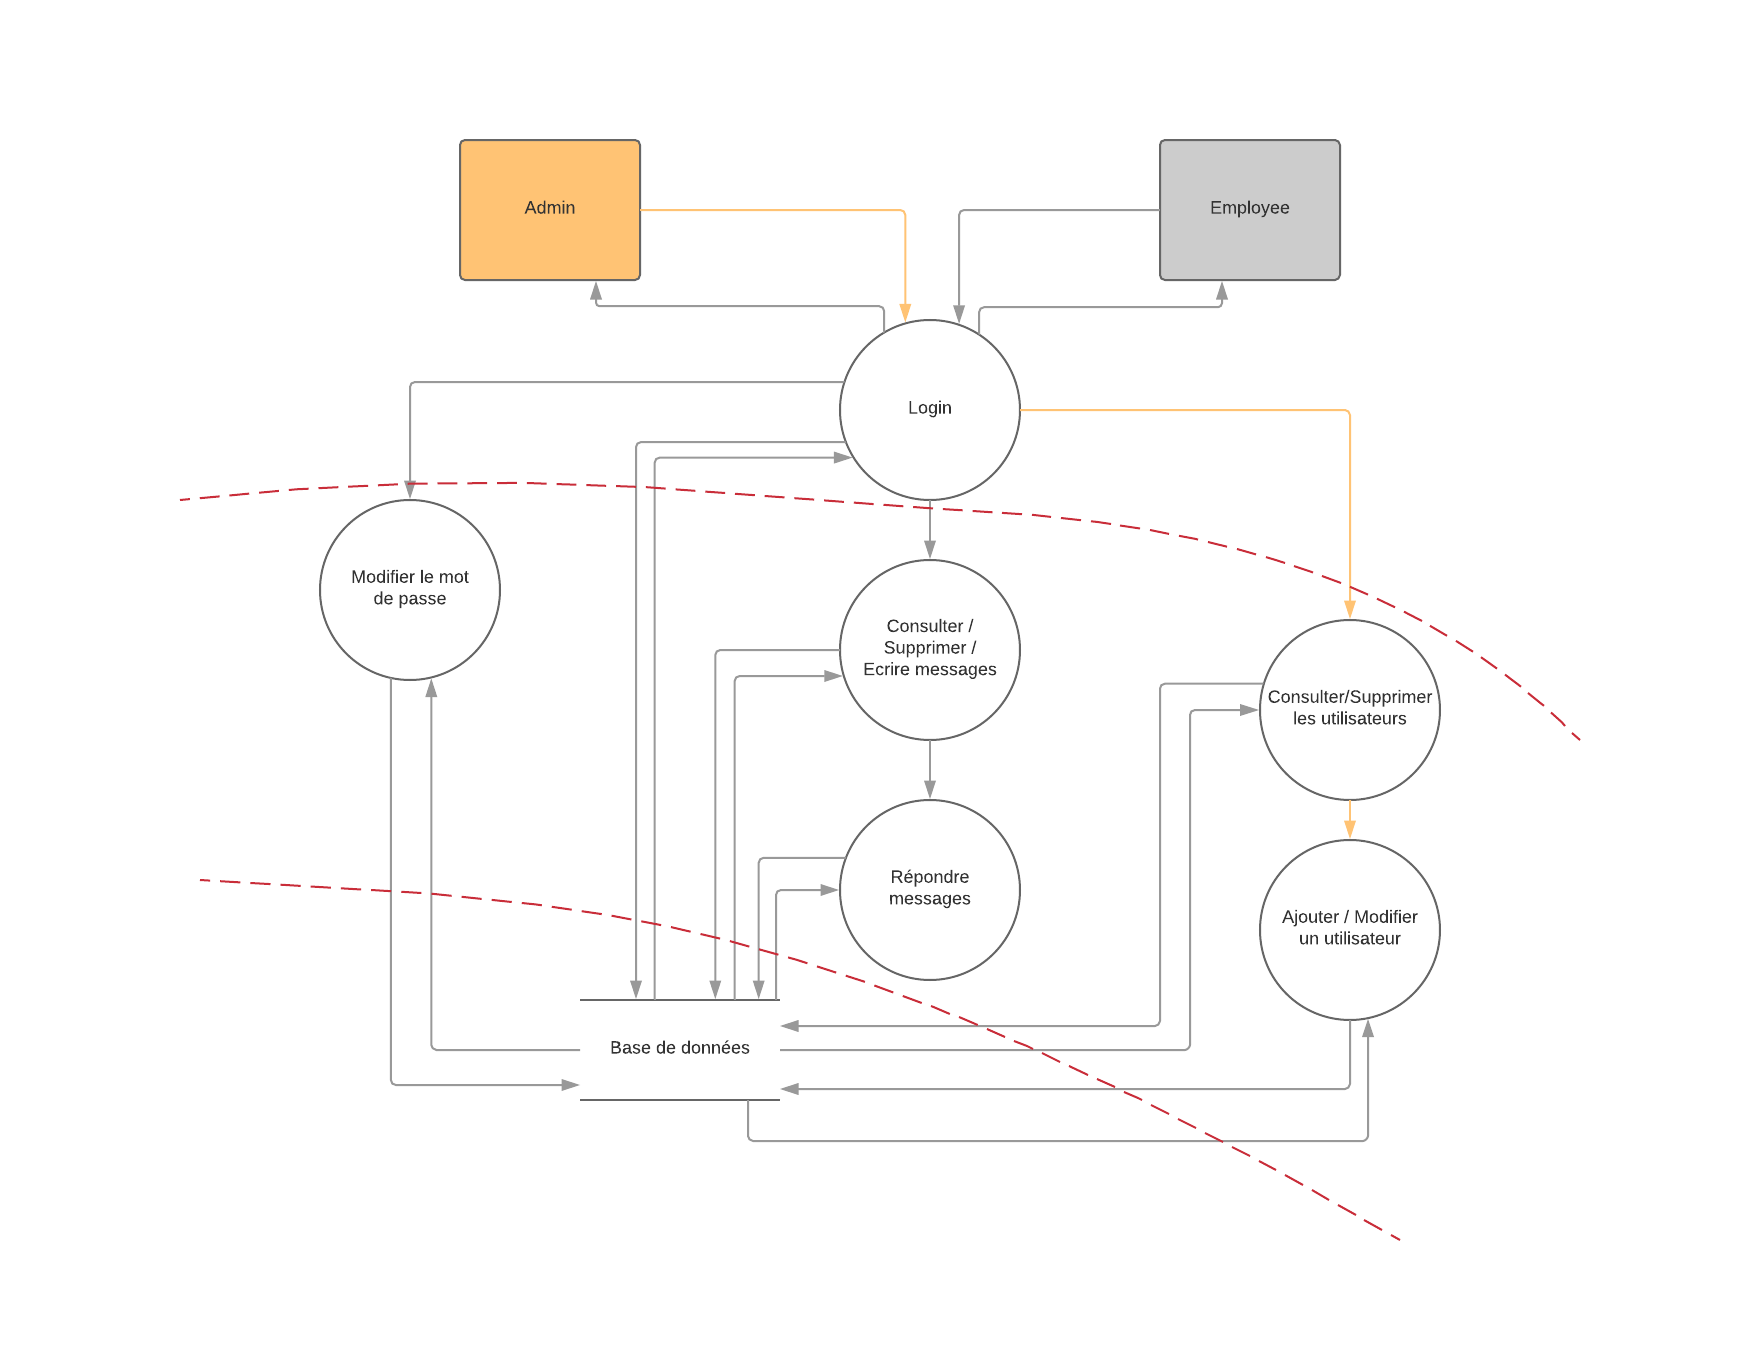
\includegraphics[width=\textwidth]{images/dfd.png}

\subsection{Périmètre de sécurisation}

Afin de pouvoir sélectionner les éléments à sécuriser, nous avons établi
une liste de priorités des différentes menaces. Les menaces se trouvant
en haut de la liste sont celles que l'ont veut éviter à tout prix, et
c'est donc ces éléments qui devront être sécurisés en premier:

\begin{enumerate}
\def\labelenumi{\arabic{enumi}.}

\item
  \textbf{Accès à la zone admin :} Cela permettrait d'ajouter/de
  modifier ou de supprimer des utilisateurs , ce qui est un gros
  problème. Le login doit donc être sécurisé au maximum. Il est aussi
  important de rechercher les failles qui permettraient d'y accéder
  autrement que par le login.
\item
  \textbf{Accès au message des autres utilisateurs :} Pour garantir la
  confidentialité, il faut être sûr d'avoir identitifé toutes les
  failles qui pourraient permettre d'y accéder.
\item
  \textbf{Message forgés :} S'il est possible de modifier l'expéditeur
  d'un message, cela pose un gros problème de confiance et
  d'authenticité.
\item
  \textbf{Modification/suppression des messages après envoi :} Egalement
  problématique, car cela peut nuire à la bonne communication dans
  l'entreprise.
\item
  \textbf{Récupération des mots de passe:} Comme cela nécessiterait
  d'abord de voler les hash, puis de retrouver les mots de passe
  correspondant, cette menace peut être évaluée plus tard.
\end{enumerate}

\subsection{Sources de menaces}

Dans cette partie, les différents types de personnes qui pourraient
potentiellement tenter de porter atteinte au système sont énumérées.
Leurs motivation, leur cible et la potentialité qu'ils attaquent
réellement le système sont également présentés.

\subsubsection{Employés / utilisateurs malins}

\textbf{Motivation :} vengeance, espionnage industriel, curiosité

\textbf{Cible :} messages des autres utilisateurs

\textbf{Potentialité :} haute

\subsubsection{Concurrent}

\textbf{Motivation :} espionnage industriel

\textbf{Cible :} Les messages présents dans la base de données (secrets
industriels)

\textbf{Potentialité :} Moyenne

\subsubsection{Hackers, script-kiddies}

\textbf{Motivation :} défi, ego, s'amuser

\textbf{Cible :} Tout le système

\textbf{Potentialité :} Moyenne

\subsubsection{Cybercrime}

\textbf{Motivation :} financières

\textbf{Cible :} Informations des utilisateurs, spam/phishing

\textbf{Potentialité :} Moyenne

\subsection{Scénarios d'attaques}

Cette partie du rapport présente tout d'abord la méthode catégorisation
STRIDE qui sera utilisée, puis les différents scénarios d'attaque qui
ont été imaginés. Chacun de ces scénarios contient des informations
permettant de lui attribuer une priorité, ou simplement de le
catégoriser comme l'impact que l'attaque aurait, les sources de menace,
leurs motivations, les éléments attqués et les failles permettant
l'attaque. Les scénarios sont ensuite décrits en détail avec, pour
certains, une petite démonstration de l'attaque. Les contre-mesures sont
ensuite nommées. Elles seront décrites plus en détail dans le chapitre
suivant.

\subsubsection{STRIDE}

La méthode de catégorisation STRIDE permet d'identifier le but des
attaquants pour une menace donnée. STRIDE signifie:

\begin{itemize}

\item
  Spoofing
\item
  Tampering
\item
  Repudiation
\item
  Information Disclosure
\item
  Denial of Service
\item
  Elevation of Privilege
\end{itemize}

Cela permet également de savoir comment contrer les menaces, chaque
catégorie ayant un type de contrôle de sécurité associé:

\begin{itemize}

\item
  Spoofing -\textgreater{} Authentication
\item
  Tampering -\textgreater{} Integrity
\item
  Repudiation -\textgreater{} Non-Repudiation
\item
  Information Disclosure -\textgreater{} Confidentiality
\item
  Denial of Service -\textgreater{} Availabiliy
\item
  Elevation of Privilege -\textgreater{} Authorization
\end{itemize}

De manière générale, cela permet de catégoriser les menaces afin d'avoir
une meilleure vue d'ensemble.

\subsubsection{Scénario 1 : Guessing de mot de passe}

Etant donné qu'il est nécessaire d'être authentifié pour avoir accès aux
fonctionnalités de l'application, ce scénario est une première étape
permettant ensuite de pouvoir lancer d'autres attaques. Les scénarios 2
et 3 présentent d'autres manières de s'authentifier illégalement.

\textbf{Catégorie STRIDE:} S (Spoofing)

\textbf{Impact:} Haut (permet d'effectuer d'autres attaques)

\textbf{Source de menace:} Hacker, Cybercrime, Concurrents, Employés

\textbf{Motivations:}

\begin{itemize}

\item
  Pour les hackers, cela peut être un défi en soi ou un moyen d'accéder
  à plus de défis.
\item
  Pour des cybercriminels ou des concurrents, l'intérêt est d'avoir
  accès au système de messagerie.
\item
  Pour les employés, le but peut être de se faire passer pour quelqu'un
  d'autre, de lire les messages de quelqu'un d'autre ou d'utiliser des
  fonctionnalités réservées aux administrateurs.
\end{itemize}

\textbf{Element(s) du système attaqué:} Informations des utilisateurs
(login/password)

\textbf{Faille(s) permettant l'attaque:} * Aucune vérification sur les
mots de passe choisis * Mots de passe définis par l'admin

\textbf{Scénario d'attaque:}

Lorsqu'on crée un utilisateur ou que l'on change son mot de passe, il
n'est pas demandé de fournir un nombre minimum de caractères ou
d'utiliser des chiffres et des signes de ponctuation. Il n'y a pas non
plus d'avertissement rappelant à l'utilisateur de ne pas choisir un mot
de passe trop simple. Il est donc fort possible qu'un grand nombre
d'utilisateur choisissent comme mot de passe leur login ou quelque chose
comme 1234. Dans la situation actuelle, tester les mots de passe
suivants permet d'accéder à tous les comptes : - Login (p.~ex : admin ou
lucie) - 1234 - 12345678 - Abcd Une autre faiblesse actuelle est que
seuls les administrateurs peuvent créer des nouveaux utilisateurs.
L'avantage est que cela empêche des personnes externes de se créer un
compte, mais l'inconvénient est que les administrateurs doivent mettre
un mot de passe par défaut, que les utilisateurs sont censés modifier
par la suite. Dans la réalité, le mot de passe par défaut sera souvent
quelque chose de simple, pour simplifier la tâche à l'administrateur. Il
peut s'agir par exemple du login, du nom de famille, ou d'une
combinaison du prénom et du nom de famille. En ajoutant à ça le fait que
plusieurs utilisateurs ne changeront pas très rapidement, voir jamais,
tenter différentes combinaisons basées sur le nom des employés peut
donner beaucoup de résultats. Les employés de l'entreprise sont ceux qui
peuvent le mieux exploiter cette faiblesse, étant donné qu'ils
connaissent la logique de choix des mots de passe.

\textbf{Contre-mesures:}

\begin{itemize}

\item
  Forcer les utilisateurs à choisir un mot de passe fort (au moins 8
  caractères, lettres et chiffres, maj/min)
\item
  Ajouter une recommendation (" Le mot de passe ne doit pas contenir
  votre login, votre nom ou prénom, le nom de l'entreprise ou de
  l'application. Si possible, choisissez un mot de passe qui n'a pas de
  sens. ``)
\item
  Pour les administrateurs : Générer un mot de passe aléatoire pour les
  nouveaux utilisateurs et le leur communiquer de manière sécurisée.
\end{itemize}

\subsubsection{Scénario 2 : Bruteforce de mot de passe}

Cette attaque permet, comme la précédente, d'accéder aux fonctionnalités
de l'application, mais elle demande plus de compétences.

\textbf{Catégorie:} S (Spoofing)

\textbf{Impact:} Haut (permet d'effectuer d'autres attaques)

\textbf{Source de menace:} Hackers, Concurrents, Cybercrime. Les
employés peuvent également être une source de menace s'ils ont plus de
compétences qu'un utilisateur standard.

\textbf{Motivations:} * Pour les hackers, cela peut être un défi en soi
ou un moyen d'accéder à plus de défis. * Pour des cybercriminels ou des
concurrents, l'intérêt est d'avoir accès au système de messagerie. *
Pour les employés, le but peut être de se faire passer pour quelqu'un
d'autre, de lire les messages de quelqu'un d'autre ou d'utiliser des
fonctionnalités réservées aux administrateurs.

\textbf{Element(s) du système attaqué:} Informations des utilisateurs
(login/password)

\textbf{Faille(s) permettant l'attaque:}

\begin{itemize}

\item
  Une tentative de login prend très peu de temps, il est donc possible
  d'en faire beaucoup très rapidement.
\item
  Le nombre de tentatives n'est pas limité.
\item
  Le login est fait en une seule étape, très simple à automatiser.
\end{itemize}

\textbf{Scénario d'attaque:}

Une personne malveillante peut utiliser un outil pour tenter de se
connecter en testant un grand nombre de combinaisons de caractères avec
un outil approprié. Le fait que le nombre de tentatives ne soit pas
limité et que le processus de login est très simple permet de faire
cette attaque facilement.

Ici, la puissance de cette attaque est renforcée par les failles
présentées dans le scénario précédent. Plus les mots de passe sont
longs, plus le bruteforce prendra de temps.

\textbf{Contre-mesures:}

\begin{itemize}

\item
  Limiter le nombre de tentatives par adresse IP
\end{itemize}

\subsubsection{Scénario 3: Vol de mot de passe (interception)}

Comme dans les scénarios précédents, cette attaque permet de se
connecter à l'application.

\textbf{Catégorie:} S (Spoofing)

\textbf{Impact:} Haut (permet d'autres attaques)

\textbf{Source de menace:} Employés capables d'utiliser Wireshark ou
autres personnes ayant accès au réseau interne de l'entreprise.

\textbf{Motivations:}

\begin{itemize}

\item
  Pour les employés, le but peut être de se faire passer pour quelqu'un
  d'autre, de lire les messages de quelqu'un d'autre ou d'utiliser des
  fonctionnalités réservées aux administrateurs.
\item
  Pour des cybercriminels ou des concurrents, l'intérêt est d'avoir
  accès au système de messagerie.
\end{itemize}

\textbf{Element(s) du système attaqué:} Informations des utilisateurs
(login/password)

\textbf{Faille(s) permettant l'attaque:}

\begin{itemize}

\item
  La page de login utilise http pour envoyer les requêtes qui
  contiennent les login/mot de passe de l'utilisateur.
\end{itemize}

\textbf{Scénario d'attaque:}

Les informations de login transitent en clair sur le réseau. Lorsqu'un
utilisateur se connecte à son compte, une autre personne sur le même
réseau peut sniffer le trafic et trouver le mot de pase de cet
utilisateur en clair. L'outil \emph{Wrieshark} peut être utilisé dans ce
but.

\textbf{Contre-mesures:}

\begin{itemize}

\item
  Utiliser SSL/TLS pour sécuriser la page de login.
\end{itemize}

\subsubsection{Scénario 4 : Vol de session}

Cette attaque permet d'utiliser la session d'un autre utilisateur mais
contient plus d'étapes que les scénarios précédents. Elle nécessite
notamment d'être déjà connecté à l'application.

\textbf{Catégorie:} S (Spoofing), E (Elevation of privilege)

\textbf{Impact:} Haut (permet d'autres attaques)

\textbf{Source de menace:} Hackers, Concurrents, Employés avec
suffisamment de compétences

\textbf{Motivations:}

\begin{itemize}

\item
  Pour les hackers, cela constitue un deuxième défi après s'être
  connecté au site, qui le permet de devenir admin.
\item
  Pour les concurrents, cela permet de voler la session d'un
  administrateur et de lire ses messages, mais ce n'est pas très
  discret.
\item
  Pour les employés, cela peut leur permettre d'accéder à des
  fonctionnalités réservées aux administrateurs (en prennant beaucoup de
  risques). Cela peut aussi leur permettre de se faire passer pour
  quelqu'un d'autre et de lire leurs messages.
\end{itemize}

\textbf{Element(s) du système attaqué:} Utilisateurs, messages des
utilisateurs, et potentiellement les informations des utilisateurs.

\textbf{Faille(s) permettant l'attaque:}

\begin{itemize}

\item
  Cross-site scripting (XSS) possible dans la fonction d'écriture de
  messages.
\item
  Cookies de session PHP utilisées avec la configuration de base.
\end{itemize}

\textbf{Scénario d'attaque:}

Il s'agit ici d'exploiter la faille XSS en envoyant un message à un
autre utilisateur et en y introduisant le code qui nous permettra de
voler sa session. Du code javascript peut simplement être placé dans le
sujet ou le corps d'un message:

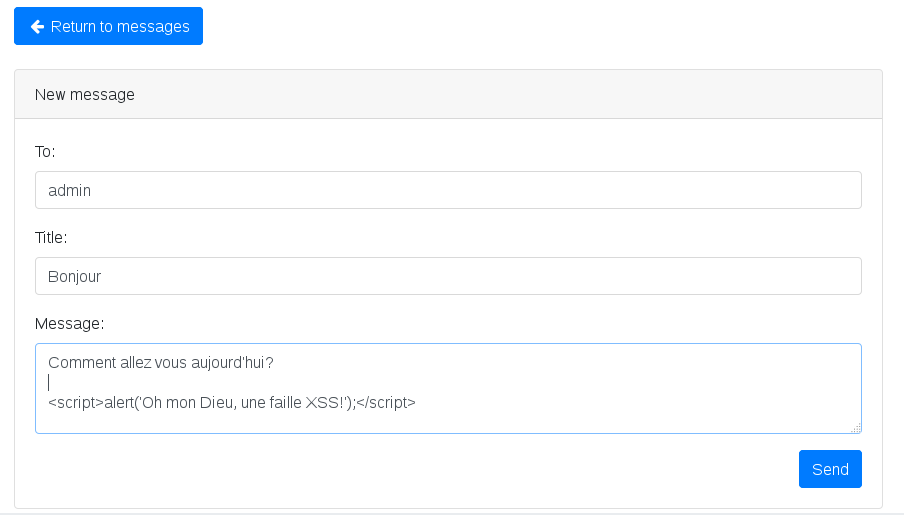
\includegraphics[width=\textwidth]{images/xss1.png}

On voit que la faille XSS est présente car lorsque le destinataire ouvre
le message, il obtient le résultat suivant:

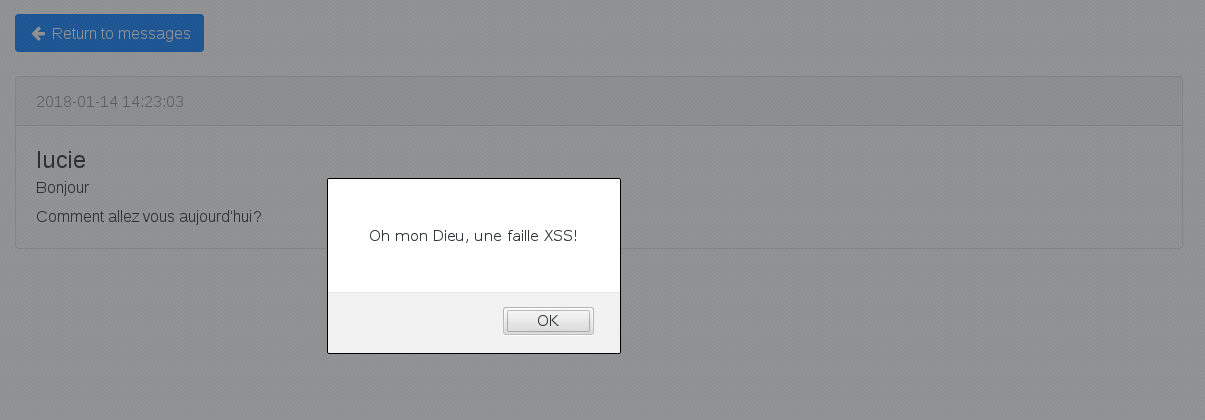
\includegraphics[width=\textwidth]{images/xss2.png}

Il s'agit ensuite d'utiliser cette faille pour récupérer le cookie de
l'administrateur. Avec Javascript, un cookie peut être affiché d'une
manière très simple:

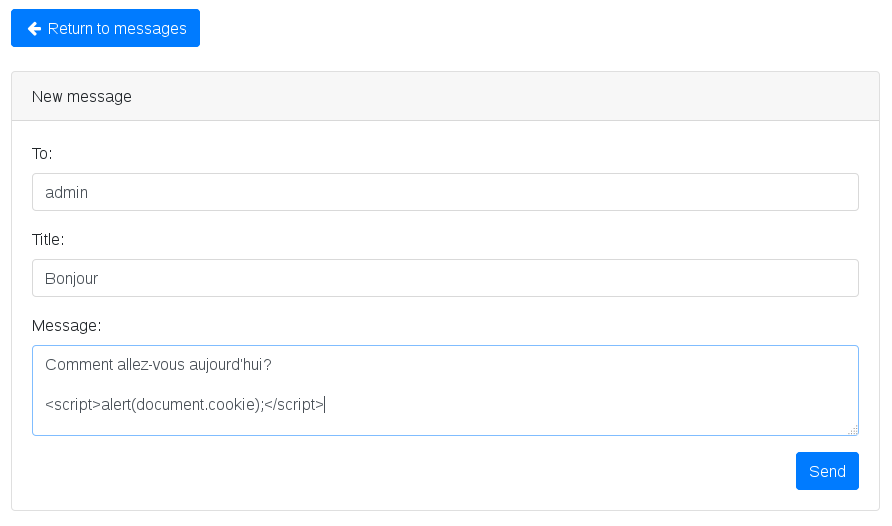
\includegraphics[width=\textwidth]{images/xss3.png}

Comme on le voit, lorsque l'utilisateur ouvre ce message, son cookie est
affiché:

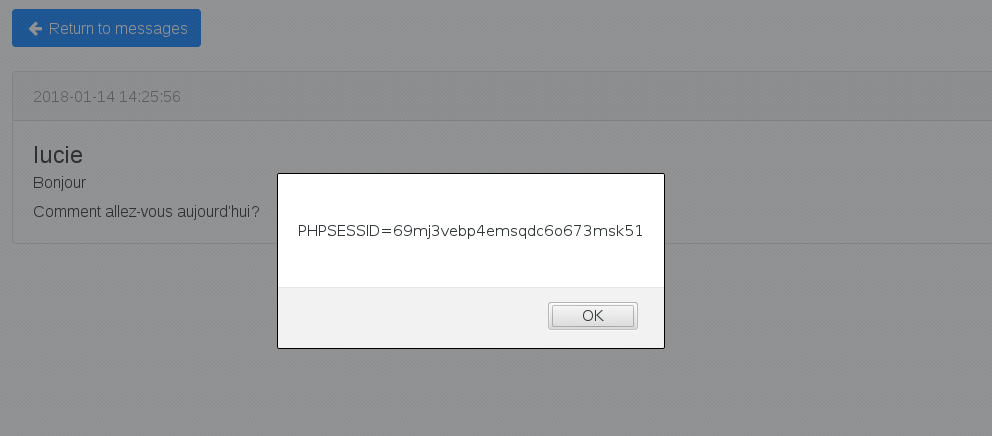
\includegraphics[width=\textwidth]{images/xss4.png}

Finalement, l'attaquant n'a qu'à envoyer ce cookie sur une page qu'il
contrôle afin de l'afficher. Cela peut être fait avec une ligne de
javascript:

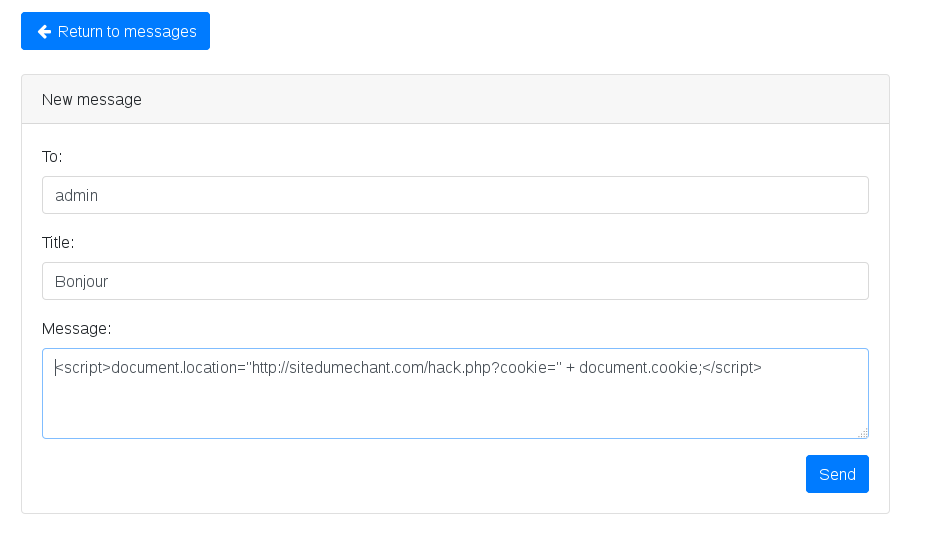
\includegraphics[width=\textwidth]{images/xss5.png}

Comme on le voit, lorsque l'administrateur ouvre le message, il
effectuera automatiquement la requête suivante:

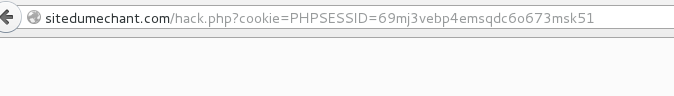
\includegraphics[width=\textwidth]{images/xss6.png}

L'attaquant aura donc reçu la requête contenant le cookie de
l'administrateur. Il n'aura donc ensuite plus qu'à remplacer la valeur
de son propre cookie par celle du cookie de l'administrateur et il aura
accès à sa session. Evidemment, un bon attaquant, fera en sorte que
l'administrateur ne se rende pas compte que cette requête a été envoyée,
mais nous ne rentrerons pas dans ces détails ici.

Le fait que le cookie de l'administrateur puisse être utilisé aussi
facilement une fois récupéré vient du fait que les cookies de session
PHP sont ici utilisés avec leur configuration de base. Ils ne sont donc
jamais modifiés avant la fin de la session et il est possible de fournir
un identifiant de session sans qu'il ait été initialisé.

\textbf{Contre-mesures:}

\begin{itemize}

\item
  Contrôler le contenu des champs ``Sujet'' et ``Message'', pour
  empêcher l'injection de code.
\item
  Refuser les id de session qui n'ont pas été initialisés avant (strict
  mode, seulement disponible à partir de PHP 5.5.2).
\item
  Régénerer l'id de session régulièrement (par exemple, lorsqu'un
  utilisateur se connecte).
\end{itemize}

\subsubsection{Scénario 5 : Mapping de l'application}

Cette attaque ne permet aucune action directe, mais elle permet d'avoir
accès à des informations qui devraient être cachées.

\textbf{Catégorie:} I (Information disclosure)

\textbf{Impact:} bas

\textbf{Source de menace:} Hackers, Concurrents, Cybercrime

\textbf{Motivations:}

\begin{itemize}

\item
  Pour tous, c'est un moyen de savoir quels fichiers existent sur le
  site, pour prévoir une autre attaque. Ce scénario est surtout
  intéressant pour les personnes externes à l'entreprise, ne connaissant
  pas le contenu du site.
\end{itemize}

\textbf{Element(s) du système attaqué:}

\begin{itemize}

\item
  Architecture de l'application
\end{itemize}

\textbf{Faille(s) permettant l'attaque:}

\begin{itemize}

\item
  Répertoires accessibles
\end{itemize}

\textbf{Scénario d'attaque:}

Il suffit d'entrer la bonne URL pour accéder directement à la liste de
fichiers contenus dans les différents répertoires. Cela fonctionne avec
les URL suivants:

\begin{itemize}

\item
  localhost/includes
\item
  localhost/models
\item
  localhost/utils
\item
  localhost/views
\end{itemize}

Lorsque l'on entre une de ces URL, ont obtient le résultat suivant:

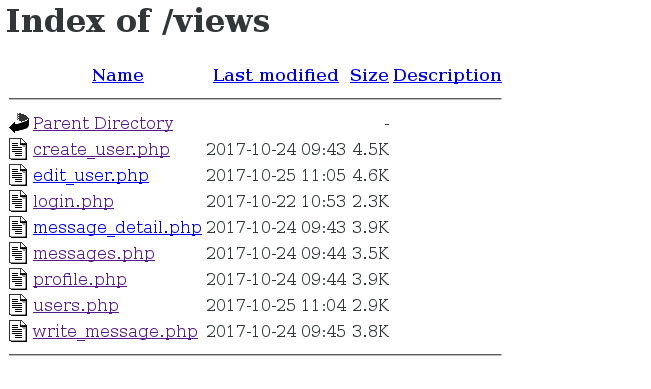
\includegraphics[width=\textwidth]{images/repertoire.png}

Les autres dossiers, contenant des fichiers définissant l'aspect du site
(css, js, vendor) sont également accessibles.

L'attaquant peut ensuite utiliser ces éléments pour se représenter
l'architecture du site, et voir quels éléments il aimerait attaquer.

\textbf{Contre-mesures:}

\begin{itemize}

\item
  Ajouter un fichier index.php à la racine des dossiers qui ne doivent
  pas être accessibles, contenant une redirection vers une autre page.
\end{itemize}

\subsubsection{Scénario 6 : Hameçonnage}

Ce scénario nécessite d'être déjà connecté à l'application.

\textbf{Catégorie:} S (Spoofing), I (Information Disclosure)

\textbf{Impact:} moyen (dépend du niveau d'information des employés)

\textbf{Source de menace:} Cybercriminels

\textbf{Motivations:}

\begin{itemize}

\item
  Leurs motivations sont principalement financières, le but est
  d'obtenir des informations qu'ils pourront revendre ou utiliser pour
  obtenir de l'argent.
\end{itemize}

\textbf{Element(s) du système attaqué:} Les utilisateurs, leur
informations de connexion ou autre (en fonction de l'objectif de
l'attaquant)

\textbf{Faille(s) permettant l'attaque:}

\begin{itemize}

\item
  Cross-site scripting (XSS) lors de l'écriture des messages
\item
  Bêtise des utilisateurs
\end{itemize}

\textbf{Scénario d'attaque:}

En utilisant la faille XSS comme cela a été décrit dans le scénario 4,
un attaquant peut ajouter du code dans un message dans le but d'afficher
à celui qui l'ouvrira une fenêtre lui demandant d'entrer certaines
informations (informations de connexion, numéro de carte de crédit ou
autre). Plus la fenêtre affichée est crédible, plus l'utilisateur sera
susceptible d'y croire et de donner des informations personnelles.

\textbf{Contre-mesures:}

\begin{itemize}

\item
  Contrôler le contenu des champs ``Sujet'' et ``Message'', pour
  empêcher l'injection de code.
\item
  Informer les employés pour leur permettre de reconnaître ce genre
  d'attaques.
\end{itemize}

\subsubsection{Scénario 7 : Suppression de messages envoyés}

Ce scénario nécessite d'être déjà connecté à l'application.

\textbf{Catégorie:} R (Repudiation) / T (Tampering) / E (Elevation of
privilege)

\textbf{Impact:} bas si utilisé de façon isolée, moyen si utilisé de
manière intensive (voir scénario 9)

\textbf{Source de menace:} Employés avec suffisamment de compétences

\textbf{Motivations:}

\begin{itemize}

\item
  Faire en sorte que le destinataire ne voie pas le message qu'on lui a
  envoyé (pour des raisons diverses).
\end{itemize}

\textbf{Element(s) du système attaqué:} La base de données, plus
précisément les messages stockés dedans.

\textbf{Faille(s) permettant l'attaque:}

\begin{itemize}

\item
  Cross-site scripting (XSS) lors de l'écriture de messages.
\end{itemize}

\textbf{Scénario d'attaque:}

Imaginons que deux employés utilisent le site de messagerie de
l'entreprise pour discuter d'une affaire illégale. Accidentellement,
l'un des deux envoie un message concernant cette affaire à leur patron.
Il doit donc trouver un moyen de le supprimer avant que son patron ne
découvre leur afffaire et les vire.

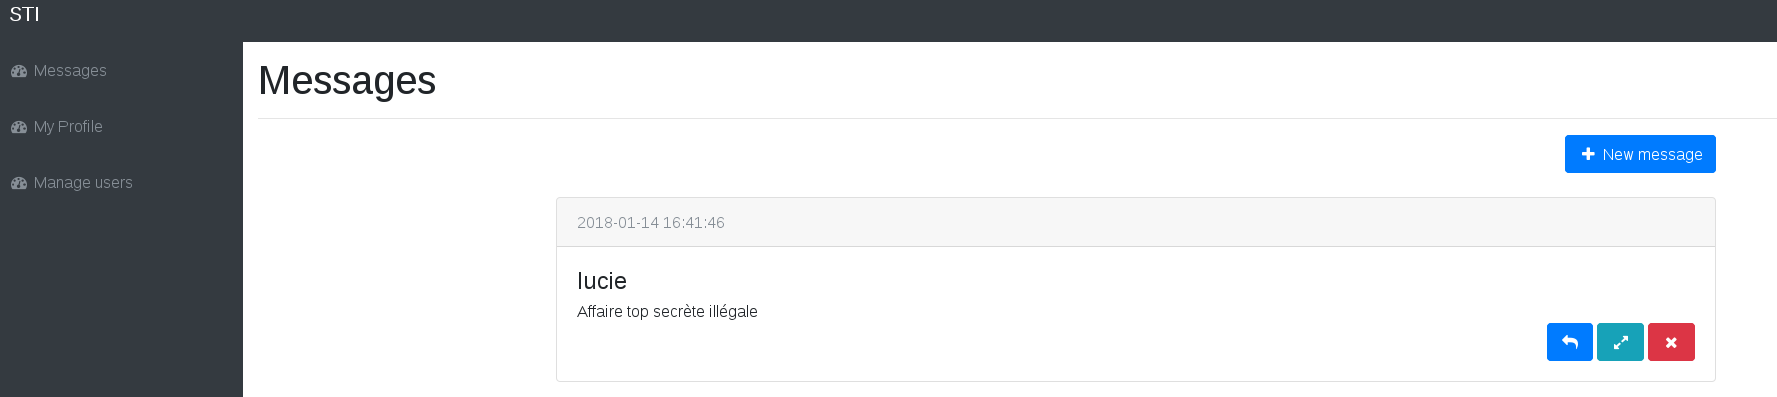
\includegraphics[width=\textwidth]{images/delete1.PNG}

L'employé en question peut supprimer ce message en envoyant un second
message au patron qui contient du code. Le code en question sera executé
du côté du patron et utilisera le fait que seul le destinataire d'un
message est autorisé à le supprimer. Ce code utilise donc les privilèges
du patron pour supprimer le premier message. Le message que l'employé
enverra à son patron pourrait être le suivant:

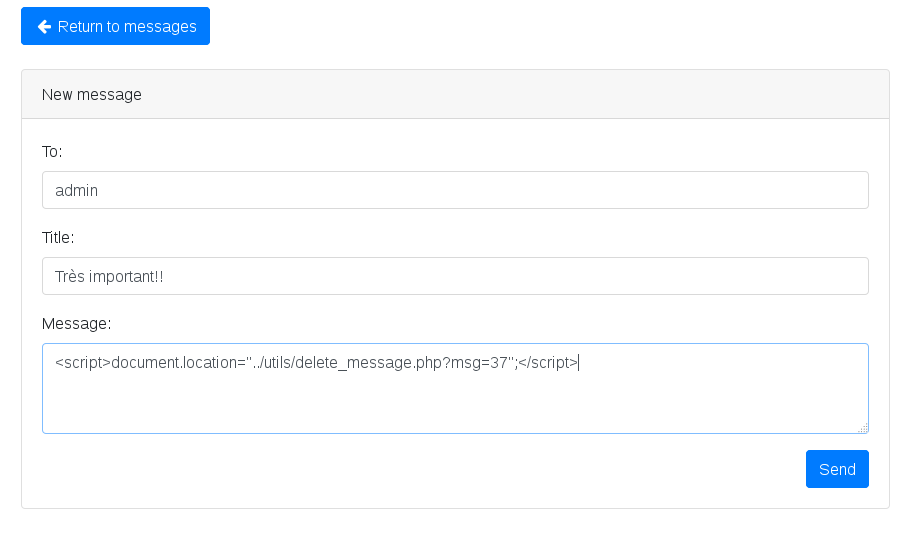
\includegraphics[width=\textwidth]{images/delete2.PNG}

\emph{Note}: On part ici du principe que l'utilisateur a un moyen de
connaître l'id des messages qu'il envoie. Comme l'id des messages est
simplement incrémenté, il peut s'envoyer un message à lui-même et en
déduire l'id du prochain message.

Lorsque le patron l'ouvre, il sera redirigé vers la page de suppresion
de message, puis de nouveau vers sa messagerie, où le premier e-mail
aura disparu:

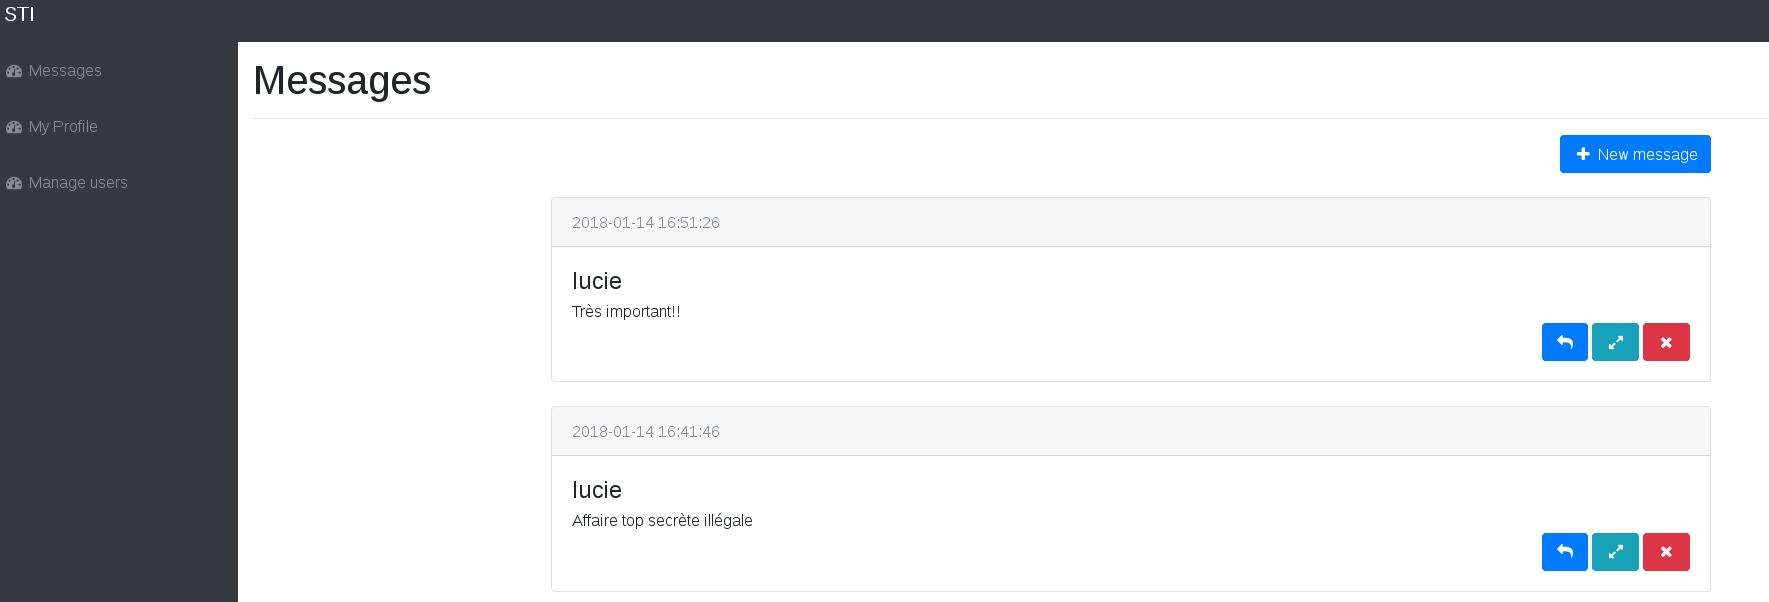
\includegraphics[width=\textwidth]{images/delete3.PNG}

Evidememnt, ce n'est pas très discret, et le patron pourrait décider
d'ouvrir d'abord le premier message. L'employé peut donc décider de
mettre son code dans le sujet du message, qui sera directement affiché:

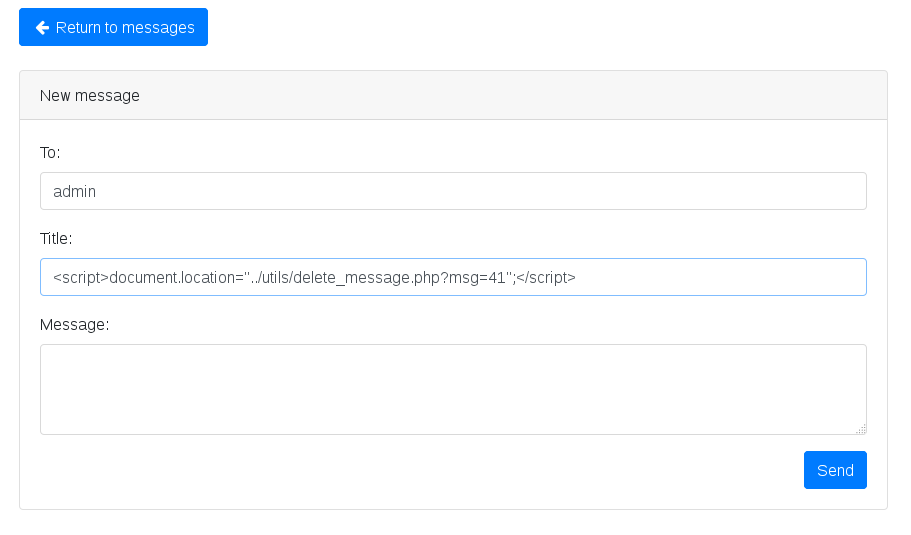
\includegraphics[width=\textwidth]{images/delete5.PNG}

Cette fois le patron sera directement redirigé vers la page de
suppression de messages en se connectant. Par contre, comme il sera par
la suite redirigé vers sa messagerie, l'employé doit également supprimer
le message contant le code pour éviter une boucle infinie de
redirection. Le message suivant devrait faire l'affaire:

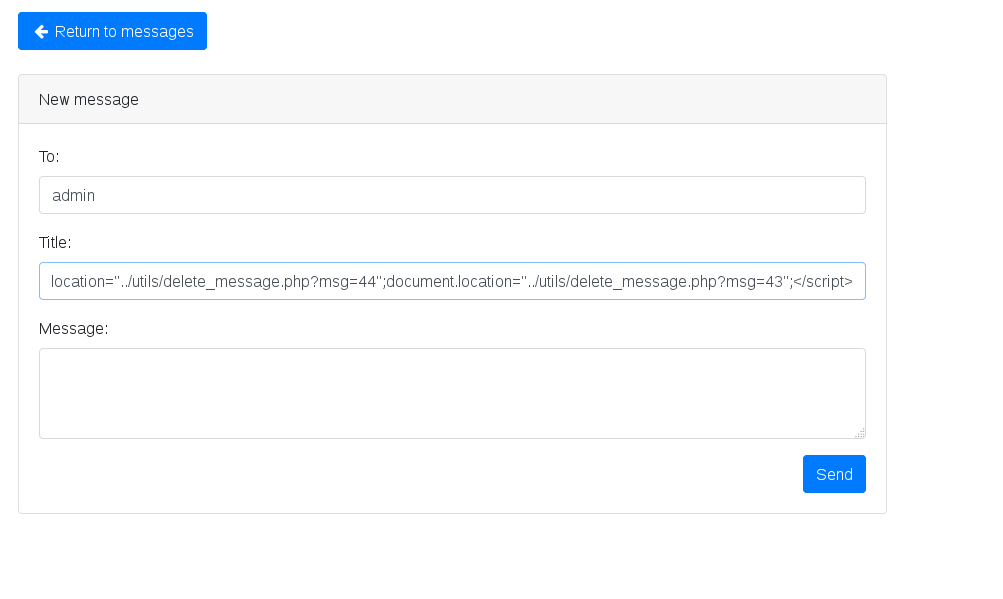
\includegraphics[width=\textwidth]{images/delete7.PNG}

Lorsque le patron ouvre sa messagerie, voici ce qu'il obtient:

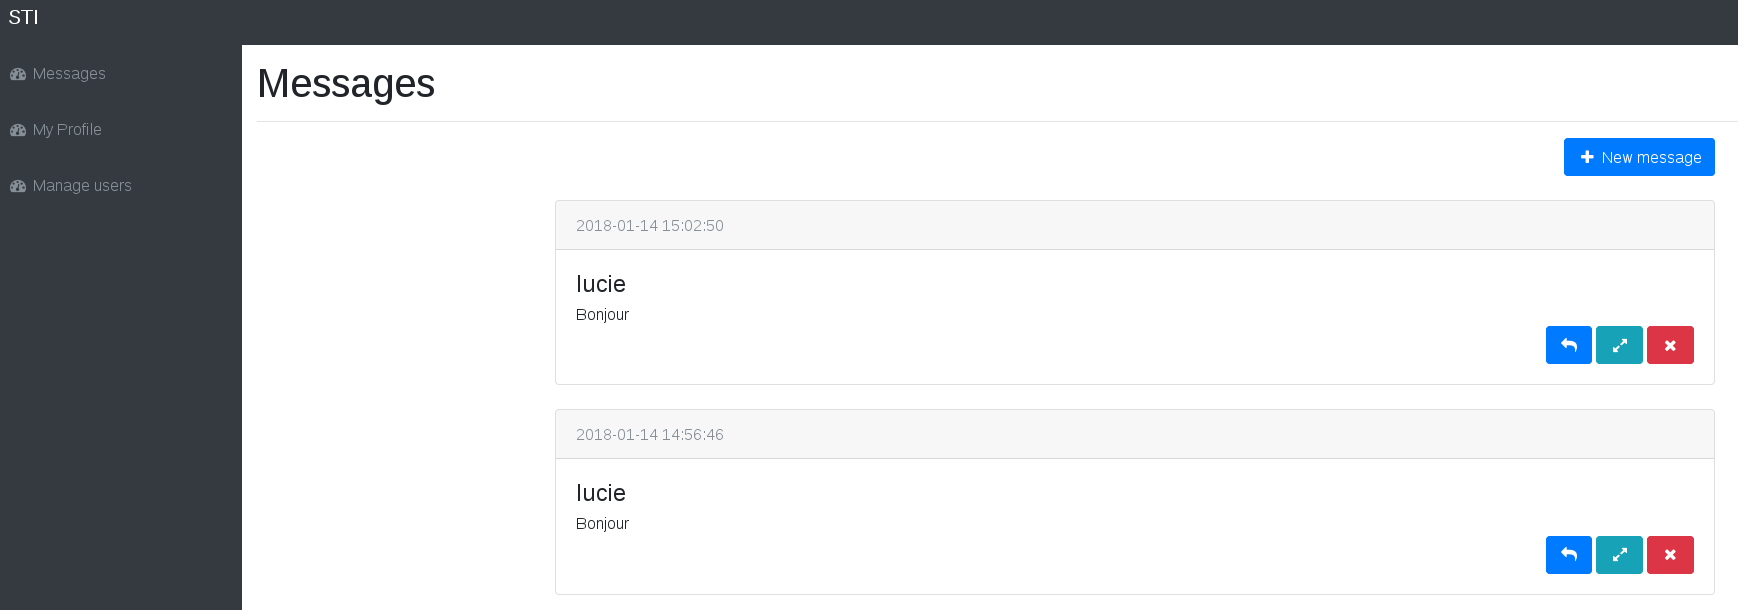
\includegraphics[width=\textwidth]{images/delete8.PNG}

Les deux messages suspects ont disparu.

\textbf{Contre-mesures:}

\begin{itemize}

\item
  Contrôler le contenu des champs ``Sujet'' et ``Message'', pour
  empêcher l'injection de code.
\end{itemize}

\subsubsection{Scénario 8 : Ralentissement de l'application}

Ce scénario nécessite d'être déjà connecté à l'application.

\textbf{Catégorie:} D (Denial of Service)

\textbf{Impact:} moyen

\textbf{Source de menace:} Employé avec des compétences suffisantes,
Hackers, Concurrent

\textbf{Motivations:}

\begin{itemize}

\item
  Pour les employés, le but peut être d'embêter un autre employé.
\item
  Pour un hacker, il peut s'agir d'un défi.
\item
  Pour les concurrents, cela peut être un moyen de perturber la
  communication dans l'entreprise.
\end{itemize}

\textbf{Element(s) du système attaqué:} Disponibilité de l'application
(pour un utilisateur)

\textbf{Faille(s) permettant l'attaque:}

\begin{itemize}

\item
  Cross-site scripting (XSS) sur la page d'écriture de message.
\end{itemize}

\textbf{Scénario d'attaque:}

Nous avons vu dans le scénario précédent comment il était possible de
faire une boucle infinie de redirection. Il suffit donc de réutiliser le
même principe, par exemple en écrivant le message suivant:

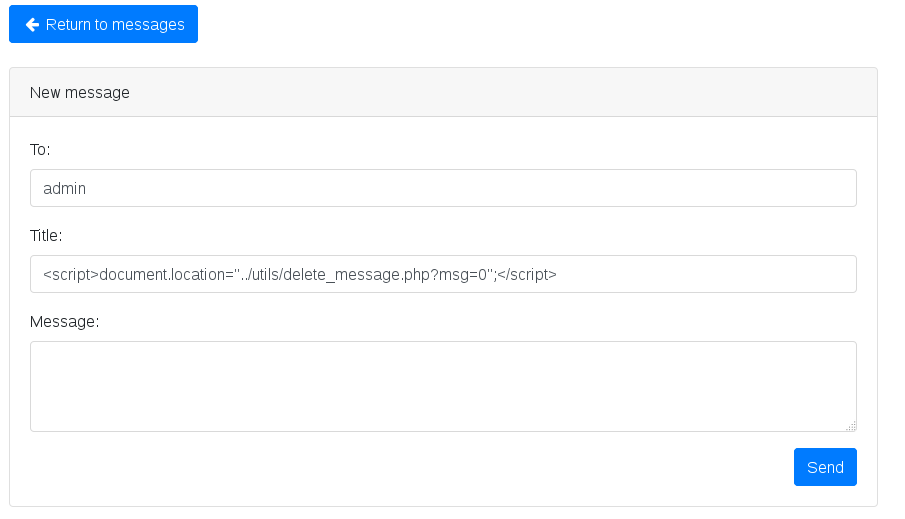
\includegraphics[width=\textwidth]{images/loop1.PNG}

Lorsque le destinataire se connectera, il sera coincé dans une boucle de
redirection l'empêchant d'utiliser la messagerie:

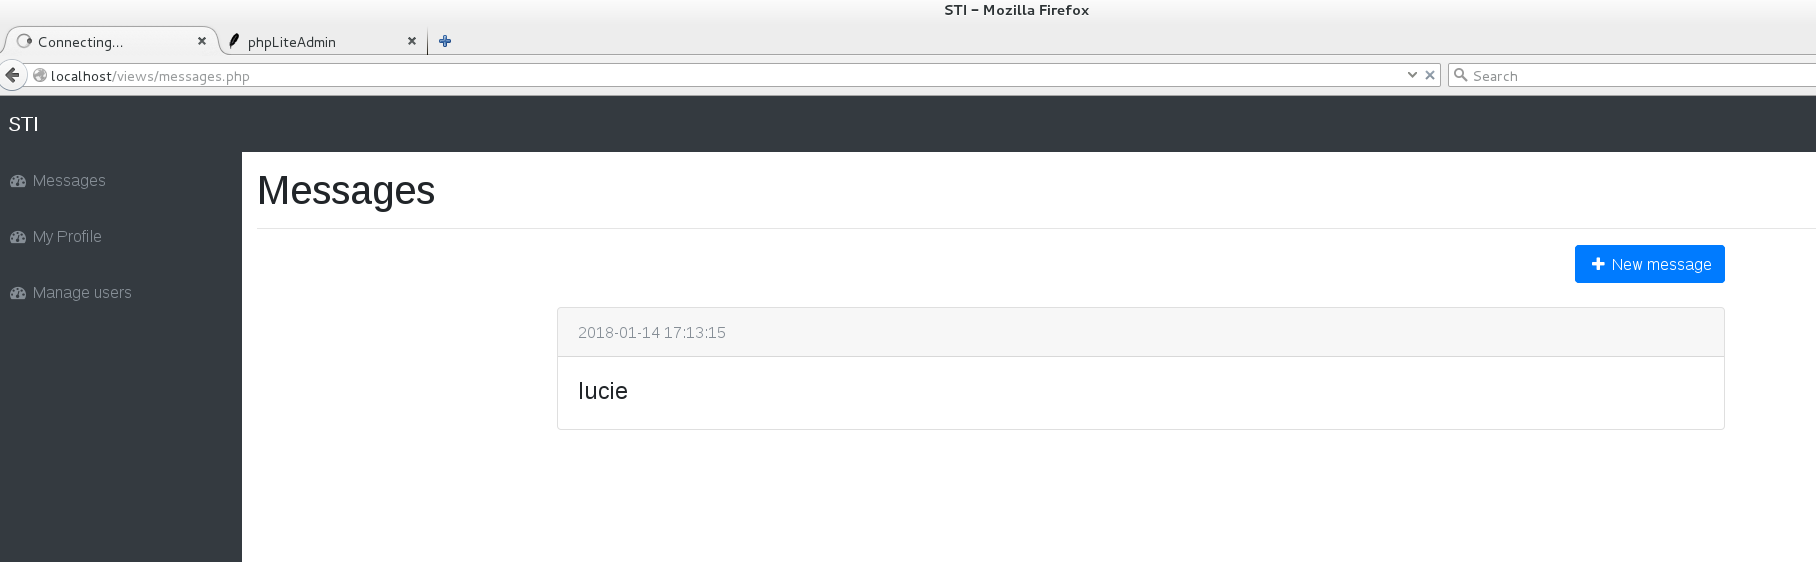
\includegraphics[width=\textwidth]{images/loop2.PNG}

\textbf{Contre-mesures:}

\begin{itemize}

\item
  Contrôler le contenu des champs ``Sujet'' et ``Message'', pour
  empêcher l'injection de code.
\end{itemize}

\subsubsection{Scénario 9 : Suppression des utilisateurs}

Ce scénario est basé sur le scénario 7. Il reprend les mêmes principes
pour une utilisation plus large.

\textbf{Catégorie:} T (Tampering)/E (Elevation of Privilege)/D (Denial
of Service)

\textbf{Impact:} haut (surtout s'il n'y a pas de backup)

\textbf{Source de menace:} Hackers, Employés mécontents avec les
compétences nécessaires, Concurrents

\textbf{Motivations:}

\begin{itemize}

\item
  Pour un hacker, le but peut être de s'amuser.
\item
  Pour un employé mécontent (ou un ex-employé) et pour les concurrents,
  le but peut être d'empêcher le bon fonctionnement de l'entreprise en
  rendant le système de messagerie inutilisable.
\end{itemize}

\textbf{Element(s) du système attaqué:} La base de données et
indirectment la disponibilité de l'application (sans utilisateur, elle
n'est pas très utile).

\textbf{Faille(s) permettant l'attaque:}

\begin{itemize}

\item
  Cross-site scripting sur la page d'écriture de message.
\end{itemize}

\textbf{Scénario d'attaque:}

De la même manière qu'un message envoyé à un autre utilisateur peut être
utilisé pour supprimer les messages de cet utilisateur, il est possible
d'utiliser un message pour avoir accès à des fonctionnalités réservées à
un administrateur. La seule qui ne nécessite pas d'étape intermédiaire
est celle de suppression d'un utilisateur.

Dans ce scénario, on imagine donc que quelqu'un veut supprimer tous les
utilisateurs de la base de données. Pour cela, il faut que
l'administrateur soit redirigé à son insu vers la page qui supprime un
utilisateur, et cela jusqu'à ce qu'il n'y ait plus d'utilisateurs. Le
code du message envoyé doit donc contenir une boucle et également
supprimer le message suspect (le message a ici été écrit dans le corps
du message pour qu'on puisse le voir en entier, mais il serait beaucoup
plus discret de le mettre dans le sujet su message):

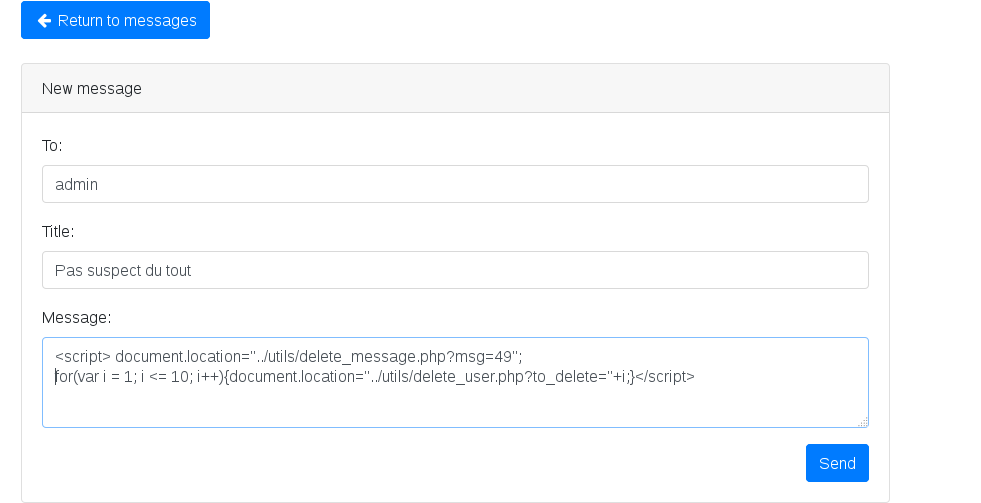
\includegraphics[width=\textwidth]{images/users1.PNG}

Lorsque l'administrateur ouvre ce message, voici le résultat:

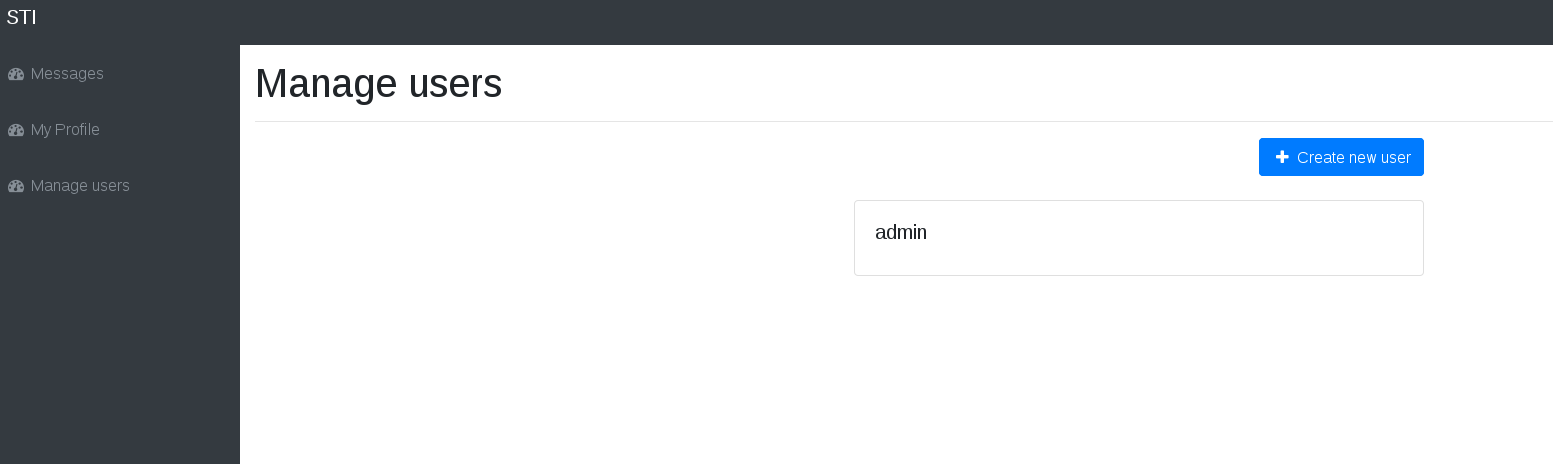
\includegraphics[width=\textwidth]{images/users2.PNG}

Etant donné que l'attaque n'est pas censée être discrète, il n'est pas
nécessaire de rediriger l'administrateur vers la page sur laquelle il
était à la base. Si on retourne sur la page des messages, le résultat
suivant apparaît:

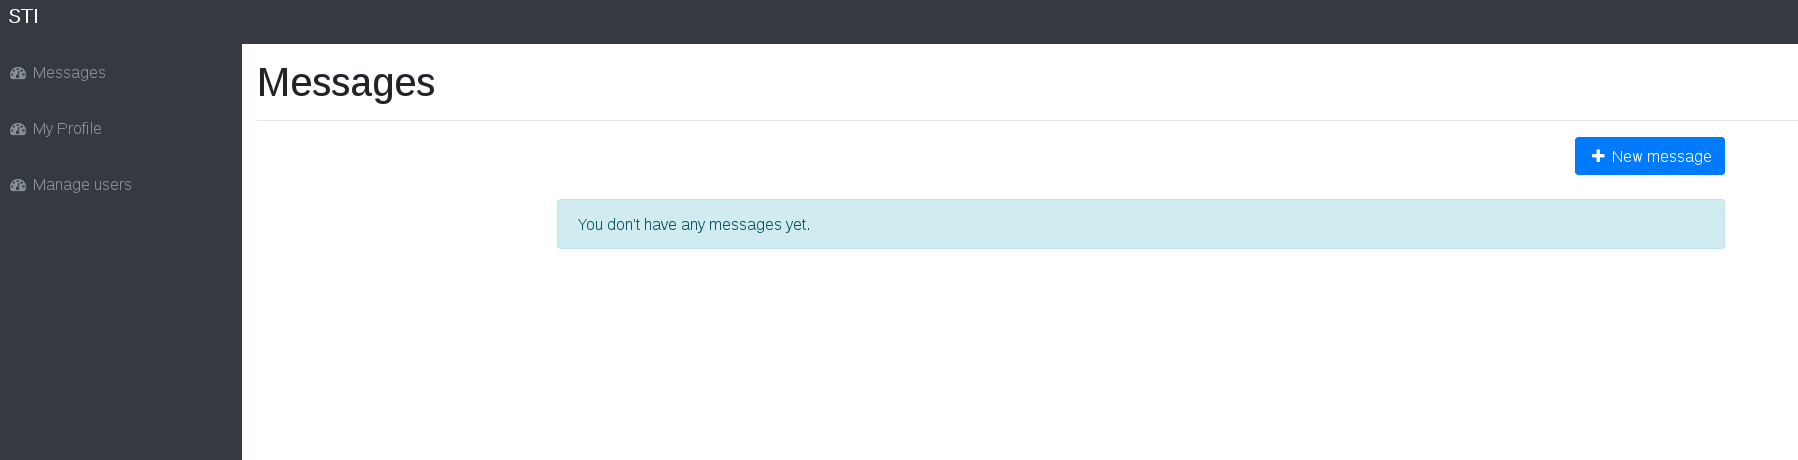
\includegraphics[width=\textwidth]{images/users3.PNG}

Plus aucun message! En réalité, ils n'ont pas été supprimés, ils ne sont
juste plus affichés, parce que les utilisateurs qui les ont envoyés
n'existent plus. Par contre, le message qui a causé la suppresion des
utilisateurs a bel et bien été supprimé, et quand la situation aura été
rétablie, il ne pourra pas être retrouvé.

\textbf{Contre-mesures:}

\begin{itemize}

\item
  Contrôler le contenu des champs ``Sujet'' et ``Message'', pour
  empêcher l'injection de code.
\end{itemize}

\subsubsection{Scénario 10: Récupération des mots de passe à partir des
hash}

Ce scénario part du principe que l'attaquant a pu obtenir les hash des
mots de passe sotckés dans la base de données par un moyen qui nous est
inconnu.

\textbf{Catégorie:} I (Information disclosure)

\textbf{Impact:} haut

\textbf{Source de menace:} Cybercrime, Hacker

\textbf{Motivations:}

\begin{itemize}

\item
  Pour les hackers, le but est seulement de s'amuser.
\item
  Pour les cybercriminels, le but peut être de revendre les mots de
  passe trouvés (les utilisateurs utilisent souvent le même mot de passe
  pour plusieurs sites) ou de les utiliser directement sur certains
  sites dans le but de gagner de l'argent.
\end{itemize}

\textbf{Element(s) du système attaqué:} Base de données, Employés et
Administrateurs

\textbf{Faille(s) permettant l'attaque:}

\begin{itemize}

\item
  Algorithme de hachage avec paramètres par défaut
\end{itemize}

\textbf{Scénario d'attaque:}

Si une manière d'accéder à la base de données nous a échappé et qu'un
attanquant est capable de récupérer les hash des mots de passe, la seule
chose qui peut l'empêcher d'obtenir les mots de passe est un algorithme
de hachage suffisamment sûr. Dans le cas de notre application, nous
avons simplement utilisé la fonction crypt(), avec les paramètres par
défaut.

La documentation de php sur la fonction crypt() nous indique que cette
fonction est faible lorsqu'elle est utilisée avec comme seul paramètre
la valeur à hacher. L'algorithme de hachage est MD5, qui est connu pour
ne plus être sûr et le salt utilisé dépend de l'implémentation.

Ces faiblesses étant connues depuis longtemps, il est probable que des
techniques pour récupérer les mots de passe à partir des hash existent
déjà (par exemple si aucun salt n'est utilisé, des rainbow tables ont pu
être calculées).

\textbf{Contre-mesures:}

\begin{itemize}

\item
  Utiliser un algorithme de hachage plus sûr (Blowfish)
\item
  Générer un sel (\emph{salt}) random lors de la création d'un nouvel
  utilisateur et le stocker avec l'utilisateur dans la base de données
\end{itemize}

\subsection{Contre-mesures}

Cette dernière partie reprend les contre-mesures qui ont été citées pour
les différents scénarios d'attaque. Elle présente leur implémentation en
détail.

\subsubsection{Mots de passe forts}

\textbf{Scénario d'attaque 1}

La force des mots de passe doit être testée sur la page de création
d'utilisateur, ainsi que sur la page de changement de mot de passe. Pour
que le mot de passe soit considéré comme fort, il doit avoir au moins 8
caractères, dont au moins une lettre minuscule, une lettre majuscule et
un chiffre. La manière la plus rapide vérifier tous ces critères est
d'utiliser un regex (source:
https://openclassrooms.com/courses/protegez-vous-efficacement-contre-les-failles-web/controlez-les-mots-de-passe).
Le code suivant a donc été ajouté dans views/create\_user.php:

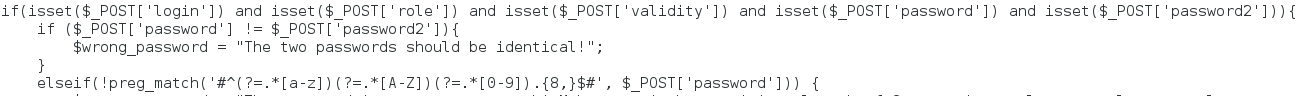
\includegraphics[width=\textwidth]{images/password.PNG}

Il a également été ajouté sur la page de changement de mot de passe,
views/profile.php:

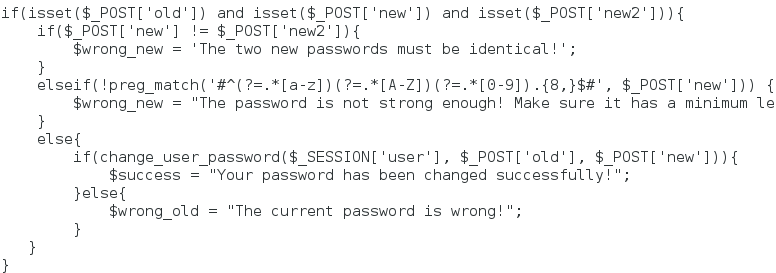
\includegraphics[width=\textwidth]{images/password3.PNG}

Comme on peut le voir, lorsqu'un mot de passe ne correspond pas à tous
les critères, un message d'erreur est affiché, rappelant les critères et
ajoutant une recommendation:

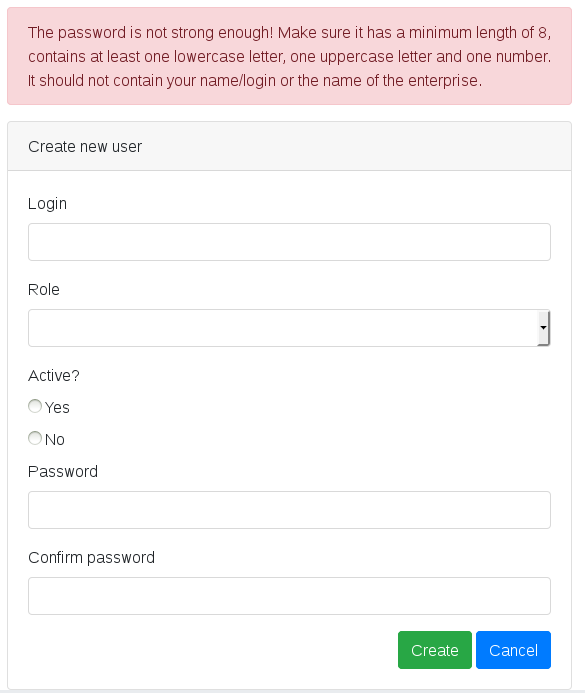
\includegraphics[width=\textwidth]{images/password2.PNG}

\subsubsection{Limiter le nombre de tentatives de login}

\textbf{Scénario d'attaque 2}

https://openclassrooms.com/courses/protegez-vous-efficacement-contre-les-failles-web/l-attaque-par-force-brute
Pour pouvoir vérifier le nombre de tentatives par adresse IP par jour,
il faut pouvoir stocker ces informations et donc ajouter une table
``connexion'' dans la base de données:

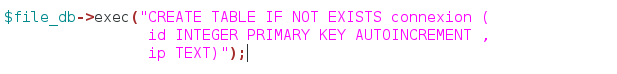
\includegraphics[width=\textwidth]{images/tentative_db.PNG}

Ensuite, il faut une fonction permettant d'ajouter des connexions et de
vérifier le nombre de connexions ayant eu lieu depuis une certaine
adresse IP ce jour-là:

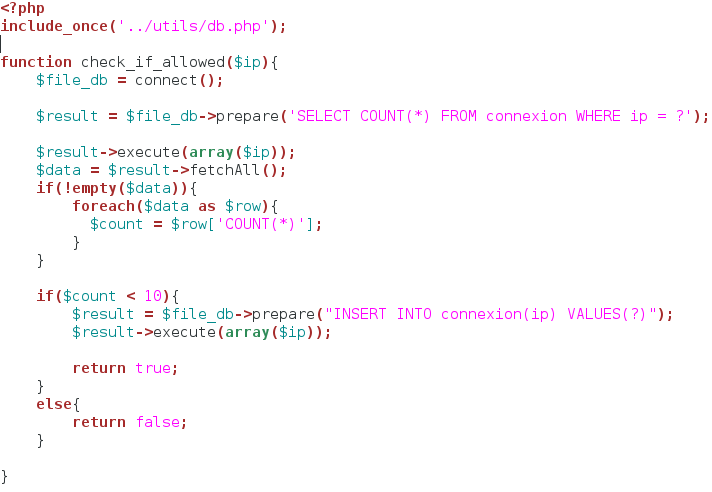
\includegraphics[width=\textwidth]{images/tentative_model.PNG}

Cette fonction compte le nombre d'occurences de l'adresse IP puis ajoute
une connexion si le nombre d'occurences est inférieur à 10. Si le nombre
d'occurences est supérieure à 10, cette adresse IP a dépassé le nombre
maximum de tentatives en 24h.

La page de login doit ensuite afficher ``Wrong credentials'' si
l'adresse IP a encore droit à des tentatives et un message informant
l'utilisateur que le nombre de tentatives maximum est atteint sinon:

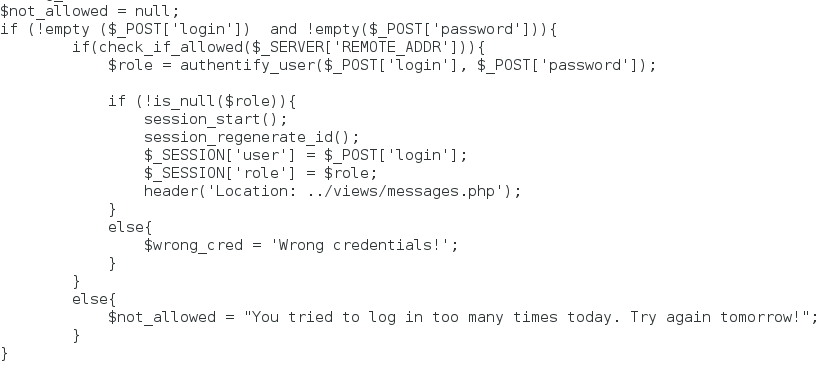
\includegraphics[width=\textwidth]{images/tentative_login.PNG}

On peut vérifier que tout cela fonctionne en entrant un mauvais
login/mot de passe plusieurs fois. En dessous de 10 tentatives, on
obtient le résultat suivant:

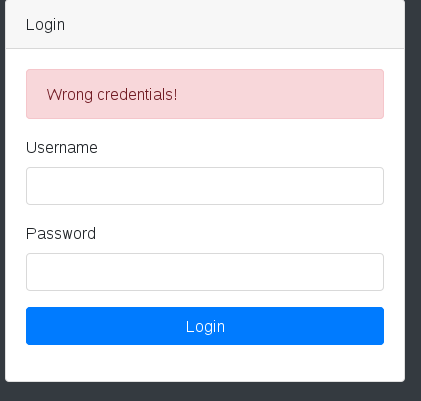
\includegraphics[width=\textwidth]{images/tentative_moins_10.PNG}

Et en dessus de 10 tentatives, le résultat suivant:

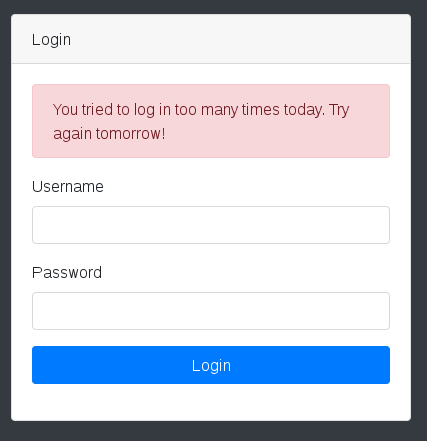
\includegraphics[width=\textwidth]{images/tentative_plus_10.PNG}

Il faut maintenant mettre quelque chose en place pour que les connexions
soient supprimées chaque jour de la base de données. Pour cela, on va
commencer par créer le script qui supprimera les connexions:

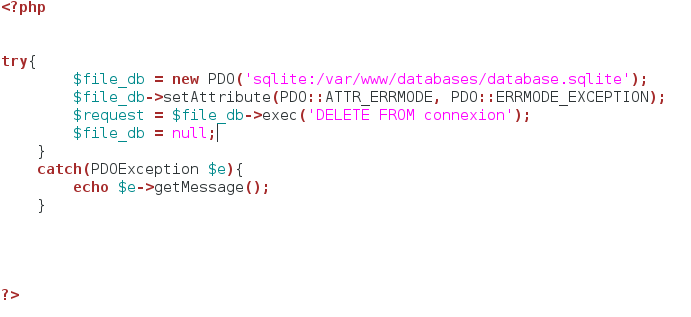
\includegraphics[width=\textwidth]{images/tentative_remove_connection.PNG}

Il est important que ce fichier ne soit pas dans l'arborescence du site,
sinon n'importe qui peut l'utiliser pour effacer les connexions. Pour la
suite des opérations, ce fichier doit être placé sur /home/sti.

Ensuite, il faut automatiser le lancement de ce script. Cela peut être
fait en utilisant \emph{cron}, qui permet de lancer une commande, par
exemple, tous les jours:

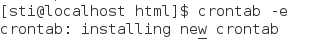
\includegraphics[width=\textwidth]{images/tentative_crontab.PNG}

Cette commande ouvre l'éditeur Vi, qu'on utilise pour ajouter la ligne
suivante:

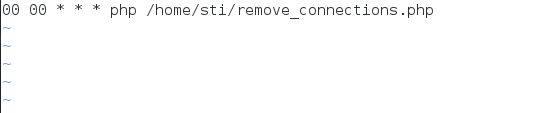
\includegraphics[width=\textwidth]{images/tentative_crontab_detail.PNG}

Cela signifie que tous les jours, à minuit, le script créé précédemment
sera appelé et les connexions seront remises à zéro.

\subsubsection{Utiliser SSL/TLS}

\textbf{Scénario d'attaque 3}

Afin de s'assurer que toutes les connections au site web sont sécurisé
en SSL/TLS il suffit de rediriger les requêtes en HTTP vers la même page
en HTTPS. Pour ce faire, il suffit de rajouter les lignes suivantes dans
le fichier \texttt{/etc/httpd/conf/httpd.conf} dans la balise
\texttt{\textless{}Directory\ "/var/www/html"\textgreater{}}

\begin{verbatim}
    RewriteEngine On
    RewriteCond %{HTTPS} off
    RewriteRule (.*) https://%{HTTP_HOST}%{REQUEST_URI}
\end{verbatim}

Ceci est possible car le serveur contient déjà un certificat autosigné
et apache est configuré pour l'utiliser. Pour un maximum de sécurité, un
certificat signé par une authorité reconnue peut être mis à la place de
ceux déjà en place dans le dossier \texttt{/etc/pki/tls/}. La clef
privée se trouve sour \texttt{private/localhost.key} et le certificat
sous \texttt{certs/localhost.crt}. Mais pour cela, un nom de domaine est
nécessaire.

Une foir les modifications effectués, le serveur doit être redémarré.
Ensuite, lorsqu'on accède à l'application, la page suivante s'affiche:

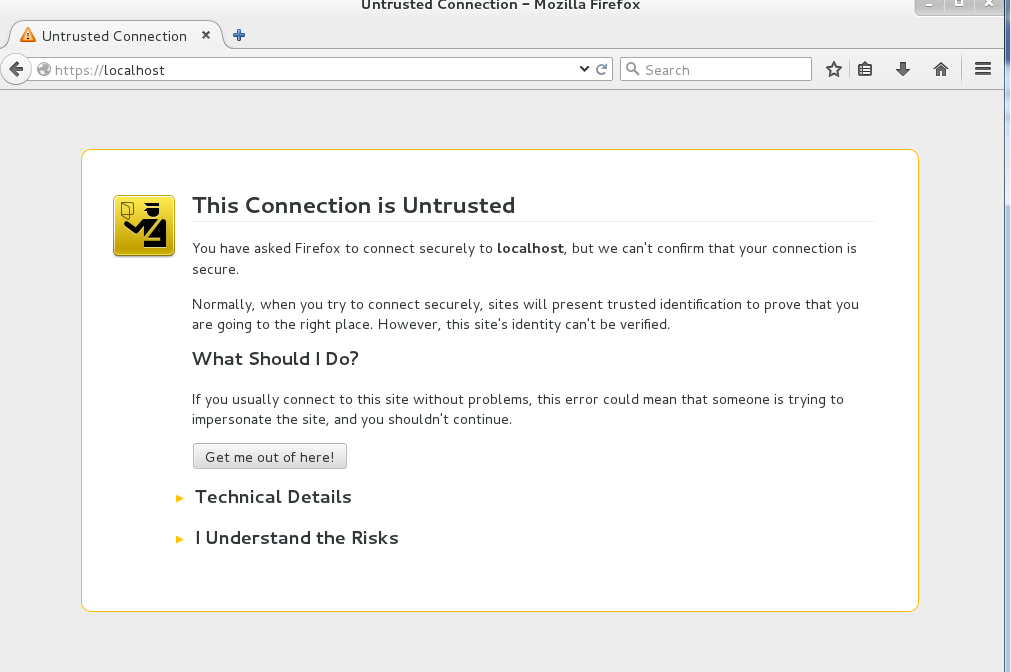
\includegraphics[width=\textwidth]{images/ssl.PNG}

Cet avertissement est normal, étant donné que le certificat est
autosigné. Il faut donc ajouter l'exception en sélectionnant ``I
Understand the Risks'', puis ``Add Exception\ldots{}'' et enfin
``Confirm Security Exception''. Il ne sera pas nécessaire de répéter
cette opération par la suite.

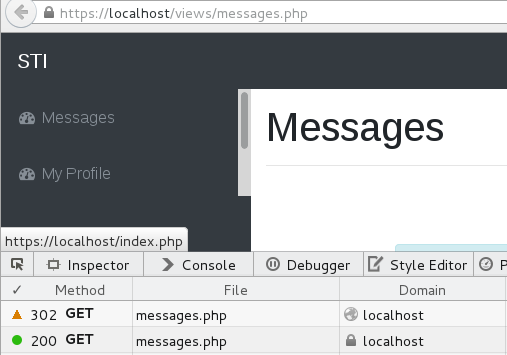
\includegraphics[width=\textwidth]{images/ssl1.png}

On peut voir que si on fait une requête sur \texttt{http://localhost/}
on est redirigé vers la version sécurisé sur laquelle le navigateur
refait la même requête et la page sécurisé est affiché comme le montre
le cadenas dans la barre d'URL.

\subsubsection{Contrôles pour empêcher XSS}

\textbf{Scénarios d'attaque 4, 6, 7, 8 et 10}

Nous avons décidé de valider les messages avant de les enregistrer dans
la base de donnée afin de pouvoir les afficher sans effort
supplémentaire. Ceci a été fait à l'aide de la fonction
\texttt{htmlspecialchars} au début de la fonction d'écriture dans la
base de donnée.

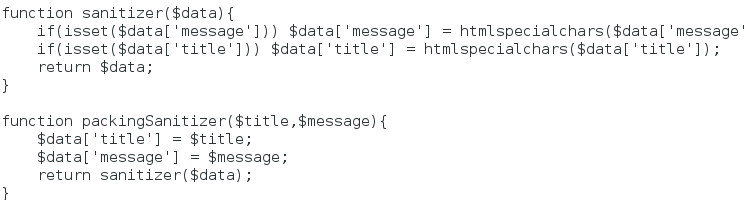
\includegraphics[width=\textwidth]{images/sanitize.PNG}
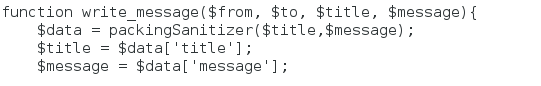
\includegraphics[width=\textwidth]{images/sanitize3.PNG}

Grâce à cette fonction, les balises et charactères spéciaux sont
échappés et affichés correctement.

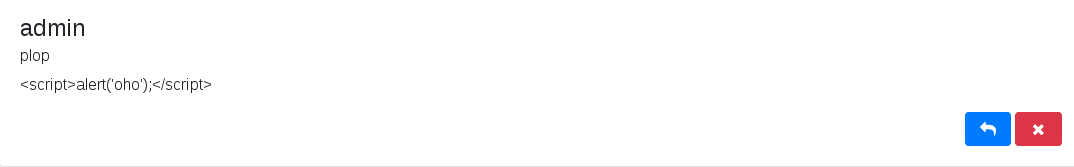
\includegraphics[width=\textwidth]{images/xss_impl1.png}

\subsubsection{Renforcer les identifiants de session}

\textbf{scénario d'attaque 4}

Un premier élément serait d'activer le \emph{strict mode}, empêchant les
utilisateurs de modifier leur identifiant de session. Malheureusement
cette otpion n'est disponible qu'à partir de PHP 5.5.2.

L'autre élément à mettre en place est de faire en sorte que
l'identifiant de session soit régénéré lorsque l'utilisateur se connecte
ou se déconnecte. Ainsi, un identifiant de session récupéré par un
attaquant ne sera pas valable longtemps. Il ne s'agit que d'une seule
ligne à ajouter dans le fichier views/login.php:

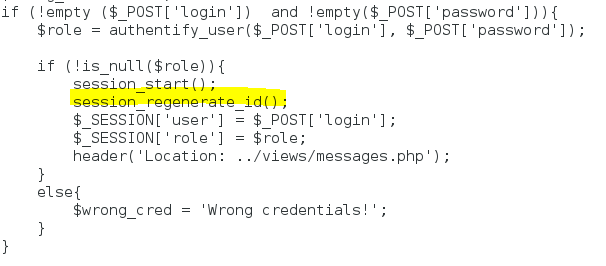
\includegraphics[width=\textwidth]{images/session_code.PNG}

la même ligne doit être ajoutée dans le fichier utils/logout.php:

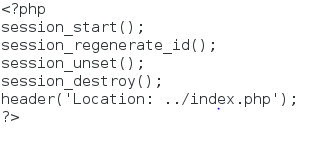
\includegraphics[width=\textwidth]{images/session_logout.PNG}

Une fois ces lignes ajoutées, on peut voir que l'identifiant de session
est modifié quand l'utilisateur se connecte:

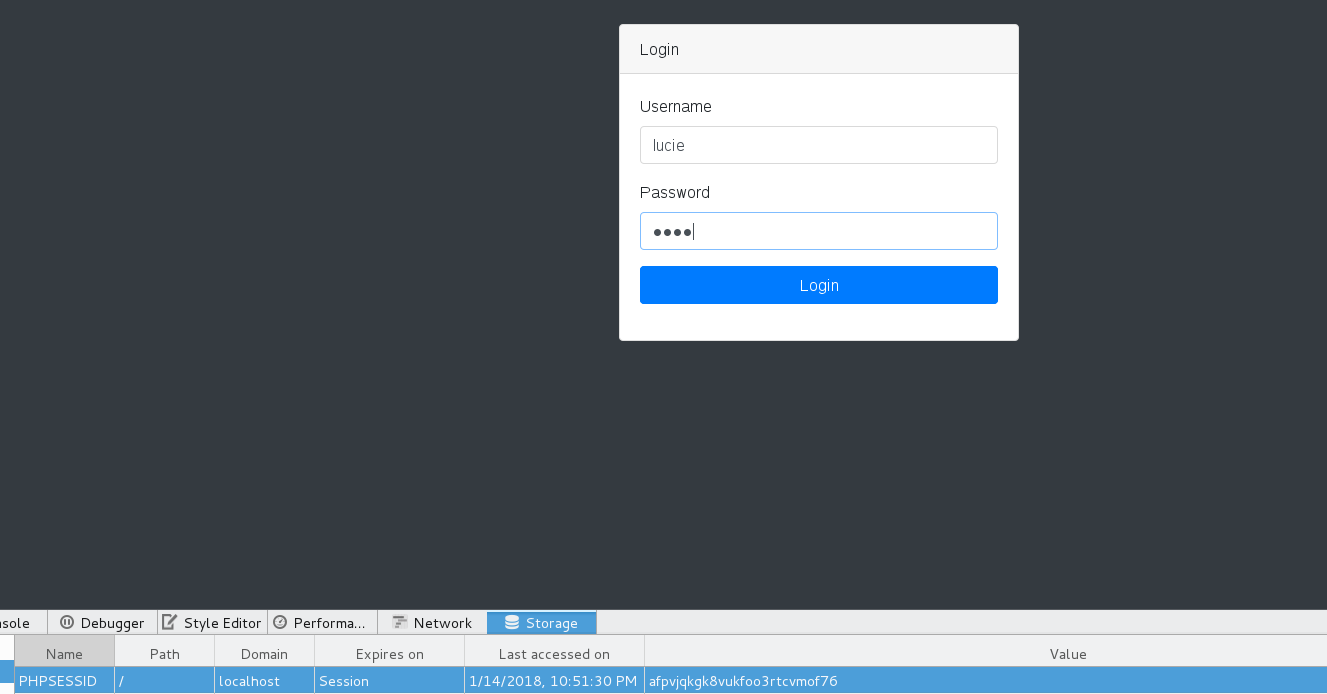
\includegraphics[width=\textwidth]{images/session1.PNG}
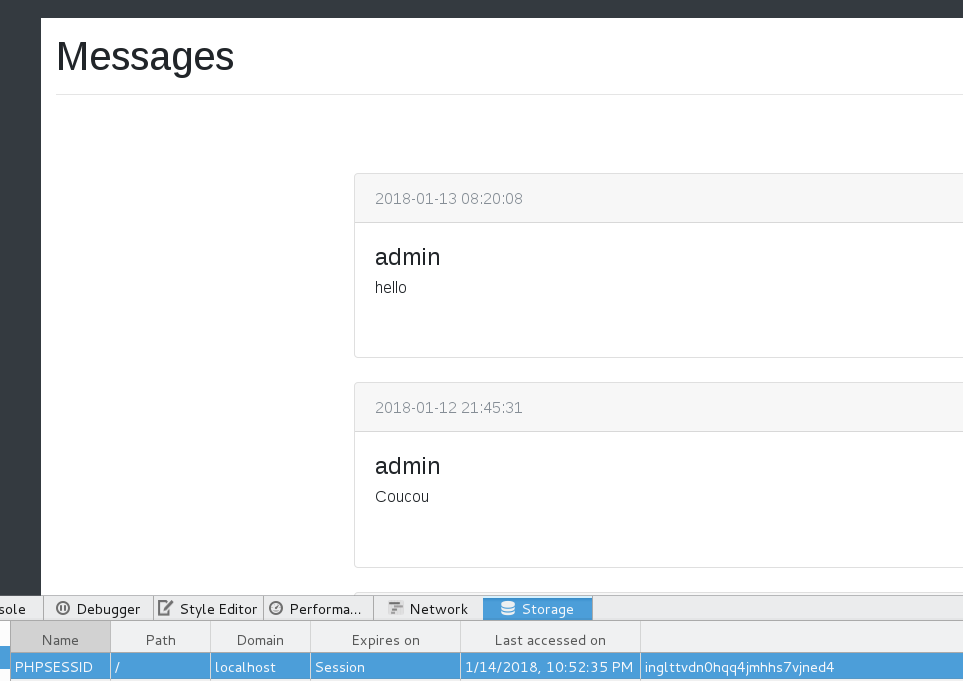
\includegraphics[width=\textwidth]{images/session2.PNG}

Le comportement est le même lorsque l'utilisateur se déconnecte.

\subsubsection{Empêcher l'accès aux répertoires}

\textbf{Scénario d'attaque 5}

Cette contre-mesure est extrêmement simple. Il suffit d'ajouter à la
racine des différents répertoires un fichier index.php qui redirige vers
une autre page:

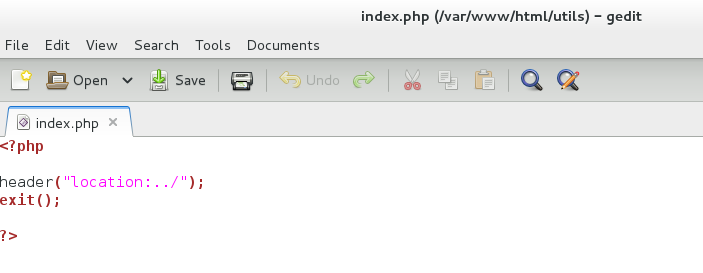
\includegraphics[width=\textwidth]{images/repertoire_fix.PNG}

https://openclassrooms.com/courses/protegez-vous-efficacement-contre-les-failles-web/protegez-vos-repertoires

\subsubsection{Renforcer l'algorithme de hachage des mots de passe}

\textbf{Scénario d'attaque 10}

L'algorithme utilisé par défaut est MD5, avec un salt dépendant de
l'implémentation. On reconnait MD5 au préfixe \(1\):

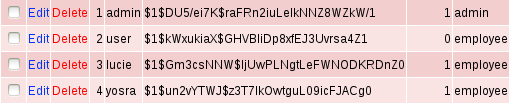
\includegraphics[width=\textwidth]{images/crypt_avant.PNG}

L'algorithme de hachage recommandé est Blowfish, avec un salt différent
pour chaque mot de passe. La partie du code contenant l'appel à la
fonction \texttt{crypt()} lors de la création d'un nouvel utilisateur
doit donc être modifiée:

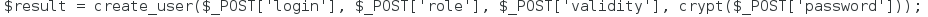
\includegraphics[width=\textwidth]{images/crypt_avant2.PNG}

Comme on le voit, actuellement il n'y a qu'un seul paramètre. pour
utiliser blowfish, il faut un deuxième paramètre (salt) avec le format
suivant: \(2a\)un nombre entre 04 et 31\$sel de 22 caractères. Cela peut
être fait au moyen du code suivant:

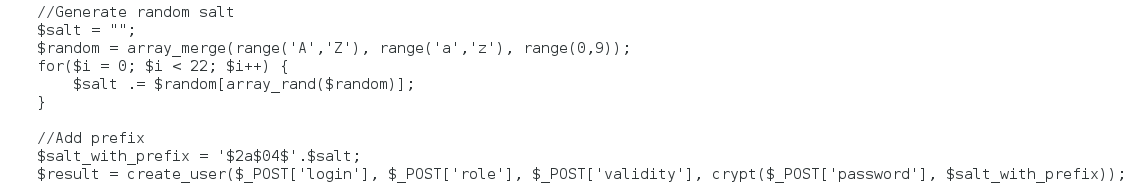
\includegraphics[width=\textwidth]{images/crypt_apres.PNG}
http://www.the-art-of-web.com/php/blowfish-crypt/

Il n'est pas nécessaire de modifier la vérification de mot de passe. La
fonction \texttt{crypt()} parse le hash pour retrouver l'algorithme
utilisé et le salt. On voit que quand on crée un nouvel utilisateur, son
hash est différent:

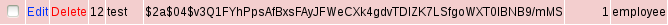
\includegraphics[width=\textwidth]{images/crypt_apres2.PNG}

On peut confirmer que tout fonctionne en se connectant avec cet
utilisateur. Le modification de l'appel la fonction crypt() doit
également être fait sur la page de changement de mot de passe:

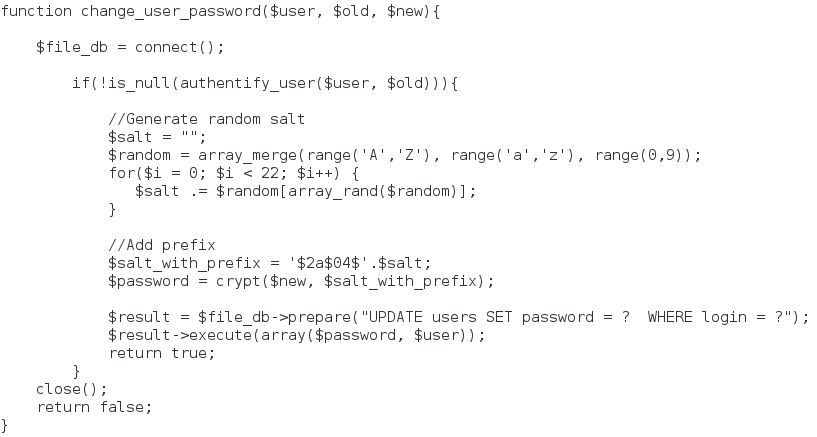
\includegraphics[width=\textwidth]{images/crypt_apres3.PNG}

Une fois cette modification faite, les utilisateurs qui modifient leur
mot de passe auront un hash plus fort:

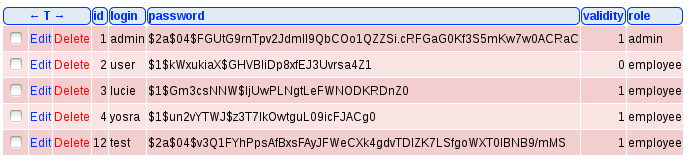
\includegraphics[width=\textwidth]{images/crypt_apres4.PNG}

Le script de création de base de données doit également être mis à jour:

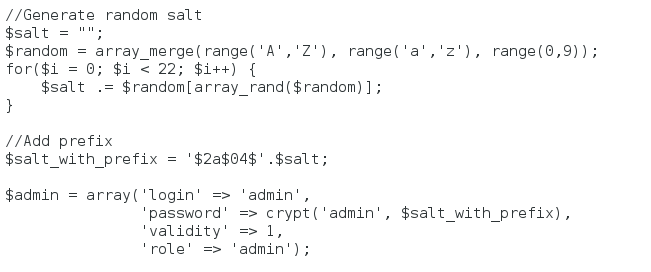
\includegraphics[width=\textwidth]{images/crypt_apres5.PNG}

\subsection{Conclusion}

Au terme de ce projet, nous avons été en mesure de sécuriser une grande
partie de l'application en appliquant des contre-mesures en fonction des
menaces relevées plus tôt. La structure de l'analyse de menaces a été
d'une grande aide pour organiser le travail.

Ce travail nous a également permis de voir quels réflexes nous avons en
matière de sécurité. En effet, l'application réalisée dans le cadre de
la première partie du projet ne devait pas être particulièrement
sécurisée, mais elle prévenait déjà de certaines attaques. Cela permet
donc aussi de mettre en évidences les réflexes que nous n'avons pas
encore, et de nous habituer à écrire du code sécurisé dès le départ.


\end{document}
